\documentclass[11pt]{article}

\usepackage[margin=1.05in]{geometry}
\usepackage{amsmath,amssymb,amsthm}
\usepackage{mathtools}
\usepackage{graphicx}
\usepackage{booktabs}
\usepackage{array}
\usepackage{microtype}
\usepackage{xcolor}
\usepackage[shortlabels]{enumitem}
\usepackage[colorlinks=true,linkcolor=blue!45!black,citecolor=blue!45!black,urlcolor=blue!45!black]{hyperref}
\hypersetup{pdftitle={Endpoint crossings for random walks with memory},pdfauthor={Arjun Pemmasani}}

% ---------- theorem environments ----------
\newtheorem{theorem}{Theorem}[section]
\newtheorem{lemma}[theorem]{Lemma}
\newtheorem{proposition}[theorem]{Proposition}
\newtheorem{corollary}[theorem]{Corollary}
\newtheorem{conjecture}[theorem]{Conjecture}
\theoremstyle{definition}
\newtheorem{definition}[theorem]{Definition}
\newtheorem{example}[theorem]{Example}
\theoremstyle{remark}
\newtheorem{remark}[theorem]{Remark}

% ---------- notation macros ----------
\newcommand{\Z}{\mathbb{Z}}
\newcommand{\E}{\mathbb{E}}
\newcommand{\Prob}{\mathbb{P}}
\newcommand{\Var}{\operatorname{Var}}
\newcommand{\CP}{\mathrm{CP}}

\title{Endpoint crossings for random walks with memory}
\author{Arjun Pemmasani}
\date{September 26, 2026}
\begin{document}
\maketitle

\begin{abstract}
Kagey asks when the middle bin of a Galton board is as likely as its ends
if the ball tends to keep its direction. For the persistent random walk,
which switches with probability $T/n$ at each step, the crossing value $z_n$
of $T$ is about $\log n$. We ask what memory changes. In the elephant random
walk each step copies a uniformly chosen earlier step and flips it with
probability $\varepsilon$. We prove that the crossing $\varepsilon_n$ is
unique and that $x_n=n\varepsilon_n$ satisfies
$x_n+\log x_n=2\log n-\log8+O((\log n)^2/n)$. So
$x_n=2z_n-\log(2\pi)+O(1/\log n)$, about twice the Markov value. For large
$n$ the law at the crossing is not unimodal. Each end is below its
neighbor, bin $n-m$ has probability about $x_n/(2m^2)$ for
$x_n\log^2x_n\ll m\ll n$, and the center is below every interior bin outside
a window of width $O(\sqrt n\log n)$. So the profile has a hump near each
end.
For alternating runs with $\Prob(\xi\ge k)=k^{-\alpha}$, $1<\alpha<2$, and a
stationary start, the ratio of end to center is of order
$n^{1-\alpha+1/\alpha}$. So the ends win for large $n$ exactly when $\alpha$
is below the golden ratio. A short remark treats aging walks, where the
crossing with a fixed first step is exactly $c=1$.
\end{abstract}

\section{Introduction}\label{sec:intro}

Suppose you drop a ball through a Galton board with $N$ rows of pegs. At the
first peg the ball goes left or right with probability $\frac12$ each. At every
later peg it repeats its previous direction with probability $p$ and switches
with probability $q=1-p$. This is the board of Problem 131 in Kagey's Open
Problem Collection~\cite{kagey131}, and one of his questions is when the middle
bin is exactly as likely as each of the two end bins. If $p$ is close to 1 the
ball rarely switches, so the ends win. If $p=\frac12$ the ball does a simple
random walk, so the middle wins. Paper~A~\cite{paperA} finds the crossing in
between. The middle catches up with the ends when the expected number of
switches $T=Nq$ is about $\log N$.

\begin{figure}[t]
\centering
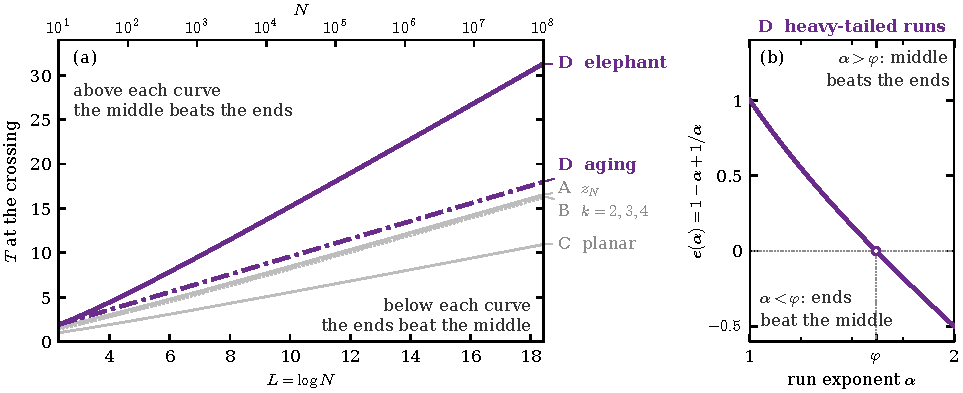
\includegraphics[width=0.8\textwidth]{../figures/program_D}
\caption{The crossing on each model's switching scale against $L=\log N$
(a), and the heavy-tailed exponent $e(\alpha)=1-\alpha+1/\alpha$ of this
paper for a stationary start (b). The scale is $T$ for Papers~A to~C,
$x=N\varepsilon$ for the elephant walk (drawn through the root $g_N$ of
Theorem~\ref{thm:erw-crossing}), and the expected number $H_N-1$ of
switches at the fixed-start crossing $c=1$ for the aging walk. The curves of
this paper are in bold, and a version of this figure also appears in
Paper~C.}
\label{fig:program}
\end{figure}

Kagey's ball remembers one step, since its next direction depends only on its
last one. In this paper we ask what happens to the middle-versus-ends question
if the ball remembers more. We study three kinds of memory.
\begin{itemize}[nosep]
\item In the elephant random walk of Sch\"utz and Trimper~\cite{schutz2004}
the ball remembers its whole past. At each peg it picks one of its earlier
directions uniformly at random and repeats it, except that with probability
$\varepsilon$ it reverses it. We write $x=N\varepsilon$, which is the expected
number of reversals up to $\varepsilon$.
\item In a walk with heavy-tailed runs the ball remembers how long it has
gone in its current direction. Its path is a sequence of runs of alternating
direction, and the run lengths $\xi$ are independent with
$\Prob(\xi\ge k)=k^{-\alpha}$ for $k\ge1$.
\item In an aging walk the ball remembers how old it is. It switches at peg
$k\ge2$ with probability $c/k$. We also give the ball $d$ directions. Then at
peg $k\ge2$ it turns to each of the other $d-1$ directions with probability
$\theta/(k+d-2)$, which is $c/k$ with $c=\theta$ when $d=2$.
\end{itemize}
The answer depends on the kind of memory. For the elephant walk the middle
needs about twice as many reversals as Kagey's board needs switches. Namely,
the crossing value of $x$ is about $2\log N$, not $\log N$. For heavy-tailed runs
started in equilibrium the ends win for large $N$ if $\alpha$ is below the
golden ratio $\varphi=(1+\sqrt5)/2$, and the middle wins if $\alpha$ is above
$\varphi$. For the aging walk with a fixed first step the crossing is exactly
$c=1$, for every $N$ and every bin. With $d$ directions the same happens at
$\theta=1$, where the vector of counts is exactly uniform
(Section~\ref{sec:aging}).

\paragraph{Why the elephant needs twice as many reversals.}
The ends are easy. The ball lands in the right end bin exactly when its first
step goes right and it never changes direction. This has probability
$\frac12(1-\varepsilon)^{N-1}\approx\frac12e^{-x}$ for the elephant walk, and
the same with $q$ in place of $\varepsilon$ for Kagey's board. So only the
middle differs. On Kagey's board the $T$ switches are spread over the whole
walk, and each moves the final position by about a run length $N/T$. So the
number of right steps spreads over about $N/\sqrt T$ bins, the middle bin has
probability of order $\sqrt T/N$, and the ends lose when $e^{-T}$ falls to
about $1/N$, that is, when $T\approx\log N$.

The elephant walk spreads a reversal in a different way. A reversal at step
$t+1$ is copied by later steps, those copies are copied, and so on. The steps
that descend from it form a family, whose share of the walk behaves like the
share of one ball in P\'olya's urn started with one ball against $t$. So a late
reversal has a small family and hardly moves the ball.
To land exactly in the middle, the walk needs a family that fills half the
walk, so it needs a reversal among its first few steps. This has probability
of order $\varepsilon$, and hitting the exact middle brings another factor of
order $1/N$. So the middle bin has probability of order $\varepsilon/N=x/N^2$ (in
fact about $4x/N^2$), and the ends lose only when $e^{-x}$ falls to about
$1/N^2$, that is, when $x\approx2\log N$. More precisely, at Kagey's crossing
$\frac12e^{-T}\approx\sqrt{2T/\pi}/N$, and squaring this relation turns it
into the elephant relation $\frac12e^{-x}\approx4x/N^2$ with
$x\approx2T-\log(2\pi)$.

The small families also give the shape of the law. About $x/m^2$ reversals
have a family of $m$ steps, so the bin at distance $m$ from an end has
probability about $x/(2m^2)$ over a wide range of $m$. So the law has a hump
near each end, and the middle is where the two tails meet. Indeed, twice
$x/(2m^2)$ at $m=N/2$ is the $4x/N^2$ above.

\paragraph{Why the golden ratio.}
For heavy-tailed runs take $1<\alpha<2$, so a run has a finite mean $\mu$ but
an infinite variance. Start the walk in equilibrium, at a typical time of a
long sequence of runs. Then the first run is already in progress, and long runs
are more likely to be in progress. The chance that this run covers all $N$
steps is of order $N^{1-\alpha}$, and this is the end. For the middle, the runs
to the right and the runs to the left form two independent renewal processes,
each making about $N/(2\mu)$ runs, and the ball ends in the middle when they
meet at level $N/2$. Each process fluctuates on the scale $N^{1/\alpha}$ of a
stable law, so they meet exactly with probability of order $N^{-1/\alpha}$. Hence the ratio of end to middle is
of order $N^{1-\alpha}/N^{-1/\alpha}=N^{1-\alpha+1/\alpha}$. The exponent
vanishes when $\alpha^2-\alpha-1=0$, that is, at $\alpha=\varphi$. Below
$\varphi$ the ends win, and above $\varphi$ the middle wins. If the first run
is a fresh run instead, the end is of order $N^{-\alpha}$, a factor $N$
smaller, and the middle wins for every $1<\alpha<2$.

\subsection{Relation to Papers A, B and C}\label{sec:series}

This is the fourth of four papers on Problem 131, which we call Papers~A, B, C
and~D. Paper~A~\cite{paperA} solves Kagey's board. Paper~B~\cite{paperB}
treats $d$ directions, where the ball turns to each other direction with the
same probability. Paper~C~\cite{paperC} gives the general theory for slowly
switching chains. These three papers study Markov walks, whose next step
depends only on the current one, and their answer is that the middle (or a
face) ties with the vertices when $T$ is of order $\log N$. This paper,
Paper~D, keeps Kagey's question and changes the walk. It can be read on its
own. From the earlier papers we use only the crossing equation of Paper~A,
namely~\eqref{eq:markov-crossing} below, and we use it only to compare the
elephant crossing with the Markov crossing in Section~\ref{sec:erw}. The four
papers share the following notation.
\begin{itemize}[nosep]
\item Kagey's board has $N$ steps (Kagey's row $n$ has $N=n-1$). The first
step is left or right with probability $\frac12$, and each later step repeats
the previous one with probability $p$. We put $q=1-p$ and $u=q/p$ (the odds of
a switch).
\item $P_N(k)$ is the probability of $k$ right steps, that is, the probability
that the ball lands in bin $k$. The endpoints have $P_N(0)=P_N(N)=p^{N-1}/2$.
\item $L=\log N$, and $T=Nq$ is the expected number of switches (up to the
first step).
\item The crossing is the value of $p$ (or of $T$) at which a bin is exactly
as likely as an endpoint. For the middle bin it is $p_N$, and
$z_N=N(1-p_N)$.
\item Papers~B and~C have $d$ states. A face $F$ is a nonempty set of states,
and the vertices are the faces of size $1$. For a chain with transition matrix
$I+(T/N)Q$, $\lambda_F$ is the principal Dirichlet eigenvalue of $-Q$ on $F$,
and $K_F$ is a second-order constant.
\end{itemize}
For the elephant walk $x=N\varepsilon$ corresponds to $T$, and its crossing
$x_N$ corresponds to $z_N$. We compare the two crossings through the crossing
equation of Paper~A~\cite[Proposition~3.8]{paperA}, which says that for every
$N\ge2$
\begin{equation}\label{eq:markov-crossing}
 z_N+\tfrac12\log z_N=L+c_0+\frac1{8z_N}+O(L^{-2}),\qquad
 c_0=\tfrac12\log\tfrac\pi8,
\end{equation}
where the error term is at most $\frac1{4L^2}+\frac{L^2+L}N$ in absolute
value, and that $L/2\le z_N\le L$. As in Paper~B the start law matters. For
heavy-tailed runs it decides whether the threshold is $\varphi$ or $1$, and
for the aging walk it decides whether the crossing is exactly $c=1$.
Figure~\ref{fig:program} shows the crossings of all four papers.

\subsection{Setting and notation}\label{sec:notation}

Every walk in this paper takes $N$ steps $X_1,\dots,X_N\in\{+1,-1\}$, where
$+1$ means right. Let $A_N=\#\{i\le N:X_i=+1\}$ be the number of right steps,
and keep writing $P_N(k)=\Prob(A_N=k)$ for the probability that the ball lands
in bin $k$, now for whichever walk we study. Unless we say otherwise the first
step is fair, $\Prob(X_1=+1)=\frac12$, and the rules treat the two directions
alike, so $P_N(k)=P_N(N-k)$. We write $\Prob_+$ and $\E_+$ for probability and
expectation given $X_1=+1$. For even $N$ we put $h=N/2$ and call
$C_N=P_N(h)$ the center and $E_N=P_N(N)=P_N(0)$ the end. Whenever $C_N$
appears, $N$ is even. The crossing is the value of the parameter at which
$C_N=E_N$. All logarithms are natural, $L=\log N$,
$H_k=\sum_{j\le k}1/j$ is the $k$-th harmonic number, and $\gamma$ is Euler's
constant. Limits, $O(\cdot)$ and $o(\cdot)$ refer to $N\to\infty$, over even
$N$ when $C_N$ appears. The constants implied by $O(\cdot)$ are absolute
unless we name what they depend on.

The elephant walk (Definition~\ref{def:erw}) has the reversal probability
$\varepsilon\in(0,1)$ and $x=N\varepsilon$. Its crossing is $\varepsilon_N$,
and $x_N=N\varepsilon_N$. Heavy-tailed runs (Section~\ref{sec:heavy}) have
the exponent $\alpha$, the mean run length $\mu=\E\xi=\zeta(\alpha)$ for
$\alpha>1$, and the length $D$ of the first run. A fresh start has $D$
distributed as $\xi$, and the stationary start has
$\Prob(D=d)=\Prob(\xi\ge d)/\mu$. We put $R_N=E_N/C_N$, so the ends win
exactly when $R_N>1$. The aging walk (Section~\ref{sec:aging}) has the
constant $c\in(0,2)$, and its version with $d$ states has the constant
$\theta$ and the count vector $(n_1,\dots,n_d)$, where $n_i$ is the number of
steps in state $i$. The symbols that only one section uses are defined at the start
of that section. The letters $p$, $q$ and $u$ have their meaning for Kagey's
board only in this introduction, and later sections reuse them locally.

\subsection{Results}\label{sec:results}

\paragraph{The elephant walk.}
For every even $N\ge2$ the crossing $\varepsilon_N$ exists, is unique and is
below $\frac12$ (Proposition~\ref{prop:mlr}). The center has derivative
exactly $4/(N+2)$ at $\varepsilon=0$
(Proposition~\ref{prop:first-mutation}), and
$C_N=\frac{4\varepsilon}{N+2}(1+O(\varepsilon\log N))$ for even $N\ge64$ and
$\varepsilon(1+\log N)\le\frac1{100}$, with explicit constants
(Theorem~\ref{thm:erw-bounds}). Let $g_N$ be the root of
$g+\log g=2L-\log8$. Then $x_N=g_N+O(L^2/N)$, and so
$x_N=2L-\log L-\log16+O(\log L/L)$ (Theorem~\ref{thm:erw-crossing}). Compared
with Kagey's board, $x_N=2z_N-\log(2\pi)+c_*/L+O(\log L/L^2)$ with
$c_*=\frac12\log(2\pi)-\frac14$ (Theorem~\ref{thm:erw-markov}).

We also go one order further. In the same range of $\varepsilon$ the center
is $\frac{4\varepsilon}{N+2}N^{2\varepsilon}(1+O(\varepsilon))$, with
explicit constants (Proposition~\ref{prop:second-order}). This gives
$x_N=g_N-(2g_NL+g_N^2/2)/(N(1+1/g_N))+O(L/N)$, so the root $g_N$ is above the
crossing for large $N$ (Proposition~\ref{prop:refined}). At fixed $N$ the
center is a polynomial $c_1\varepsilon+c_2\varepsilon^2+\cdots$ in
$\varepsilon$, and $c_2/c_1-2L\to2\gamma-2-\log2$
(Proposition~\ref{prop:K2}).

The remaining results describe the whole law near the crossing. At the
crossing the end is below its neighbor for every even $N\ge8$
(Corollary~\ref{cor:dip} and Proposition~\ref{prop:dip-hyp}). For $N<1688$
this rests on a floating-point computation whose rounding error we bound
(Lemma~\ref{lem:rounding}). Let $M_N$ be the number of steps that disagree
with the first step. For $N\ge2$ and $\varepsilon\le\frac14$ the law of $M_N$
is within an explicit $\delta_B$ of a compound Poisson law, bin by bin, and
$\delta_B=O(x^2\log^2N/N)$ when $x^2\le N$ (Theorem~\ref{thm:cp}). If
$x\to\infty$ and $x^3\log^2N/N\to0$, then $(M_N-x\log x)/x$ converges in law
to the Landau law, with a bound for each bin (Theorem~\ref{thm:landau}). So at
the crossing every mode lies at distance
$x_N\log x_N+\lambda_0x_N+O(\sqrt{x_N\log x_N})$ from the nearer end, where
$\lambda_0\approx-0.2228$ is the mode of the Landau density
(Corollary~\ref{cor:mode-location}, and Corollary~\ref{cor:modes} gives the
weaker bound $O(x_N\log^2x_N)$). Farther from the ends, bin $N-m$ has
probability $\frac x{2m^2}(1+o(1))$ for $x\log^2(x+1)\ll m\ll N$, when
$x\ge1$ and $x\log^2N/N\to0$ (Theorem~\ref{thm:profile}). Finally, for large
even $N$ the center at the crossing is below every interior bin outside a
window of width of order $N^{1/2}\log N$ around it
(Theorem~\ref{thm:shape}).

\paragraph{Heavy-tailed runs.}
For $1<\alpha<2$ and every first run that is finite almost surely, $C_N$ is
asymptotic to an explicit constant times $N^{-1/\alpha}$
(Theorem~\ref{thm:center}). With the stationary start
$R_N\sim C(\alpha)N^{1-\alpha+1/\alpha}$, and $C(\varphi)=0.7761\ldots$, so at
$\alpha=\varphi$ the center still wins. With a fresh start $R_N\to0$
(Corollary~\ref{cor:golden}). For $\alpha\ge2$ the center is of order
$N^{-1/2}$, with an extra factor $(\log N)^{-1/2}$ at $\alpha=2$, and
$R_N\to0$ with either start (Theorem~\ref{thm:alpha2}). For $0<\alpha<1$ the
runs have infinite mean and only the fresh start makes sense. Then
$NC_N\to\frac2\pi\tan\frac{\pi\alpha}2$ and $R_N\to\infty$
(Theorem~\ref{thm:lamperti}). So with a fresh start the ends win for
$\alpha<1$ and the center wins for $\alpha>1$. We do not prove what happens
at $\alpha=1$ (Remark~\ref{rem:other}).

\paragraph{Aging.}
With a fixed first step and $c=1$ the number of right steps is exactly
uniform on $\{1,\dots,N\}$. The ratio of each interior bin to the end
increases strictly in $c$, so every interior bin ties with the end exactly at
$c=1$, for every $N\ge2$ (Proposition~\ref{prop:aging-two}). With $d$ states,
a start in state~$1$ and $\theta=1$, the count vector is exactly uniform over
all compositions $(n_1,\dots,n_d)$ of $N$ with $n_1\ge1$, and every other
such bin ties with the corner $(N,0,\dots,0)$ exactly at $\theta=1$, for
every $N\ge2$ (Theorem~\ref{thm:aging-d}). A small change of the aging rate
gives a chain that redraws or repeats its state, and its counts have exactly
the law of P\'olya's urn for every weight
(Proposition~\ref{prop:aging-urn}). With a fair first step each
interior bin is twice as likely as an end at $c=1$, and its crossing is
unique and below $1$ (Proposition~\ref{prop:aging-fair}). For the center the
crossing is
$c_N=1-\log2/(\log N+\gamma+2-2\log2)+O((\log N)^{-3})$
(Proposition~\ref{prop:aging-expansion}).

\subsection{Prior work}\label{sec:prior}

The steps of the elephant walk split into clusters, since a step either
copies an earlier step exactly, with probability $1-2\varepsilon$, or starts
a new cluster with a fair sign. This is K\"ursten's coupling with bond
percolation on random recursive trees~\cite{kursten2016}, and Baur and
Bertoin~\cite{baurbertoin2016} relate the walk to P\'olya-type urns. Our
regime $N\varepsilon\asymp\log N$ lies in the strongly supercritical regime
of Baur~\cite{baur2016}, who extends the results of
Bertoin~\cite{bertoin2014} for retention probability $1-t/\log n$. Baur's
Corollary~1 gives the sizes of the largest clusters other than the root's (a
Poisson limit with intensity $a^{-2}\,da$), which is the picture of about
$x/m^2$ families of size $m$ behind Theorem~\ref{thm:profile}. These results
describe cluster sizes, not the center probability, which is a large deviation
of the root cluster. The law that appears in the bulk
(Theorems~\ref{thm:cp} and~\ref{thm:landau}) is also known. Without its
truncation, our compound Poisson law is the Lea--Coulson form of the
Luria--Delbr\"uck distribution, and Kessler and
Levine~\cite[Eqs.~(14), (18) and~(19)]{kesslerlevine2015} describe its profile
$x/(m(m+1))$ for small $x$ and its Landau limit for large $x$ (see
also~\cite{mohle2005}). The same stable law governs the fluctuations of the
root cluster when the retention probability is
$1-c/\log n$~\cite{bertoin2014ejp}. What we add is the comparison of the
elephant walk with this law in our regime (with an explicit error in
Theorem~\ref{thm:cp}) and a certified enclosure of the mode.
Gu\'erin, Laulin, Raschel and Simon~\cite[proof of Theorem~1.1]{glrs2025}
prove that the law with a fixed first step is unimodal, and their other
results fix the memory parameter as $N$ grows. So do the local limit theorem
of Trinas and Valle~\cite[Theorem~3.1]{tv2026} for the superdiffusive walk
and their bounds on where log-concavity fails. We did not find an asymptotic
formula for the center probability when $\varepsilon\to0$ as $N$ grows.

For heavy-tailed runs, Godr\`eche and Luck~\cite{godrecheluck2001} give the
transform of the occupation time of an alternating renewal process and the
scalings of the center and of both edges, and~\cite{zdk2015,dsd2013} describe
the profile of a L\'evy walk. Wang, Li and H\"anggi~\cite{wlh2016} already observe,
as a heuristic for heat conduction, that equal decay of the central peak and
the side peaks gives the golden ratio. The two decay rates of the end,
$N^{1-\alpha}$ and $N^{-\alpha}$, are the scalings of the ballistic peaks of a
L\'evy walk with and without an equilibrated start~\cite[Table~I]{dzh2012}. We
prove the lattice statement with a local limit at the center, treat both
starts, and compute $C(\alpha)$. For $\alpha<1$ the limit law of $A_N/N$ is
Lamperti's~\cite{lamperti1958}.
For aging walks, Dietz and Sethuraman~\cite{ds2007} proved the limit law of
$A_N/N$, Engl\"ander and Volkov~\cite{ev2018} gave a second proof, and
Engl\"ander, Volkov and Wang~\cite{evw2020} found the scaling limit of the
walk. For $d$ states the limit is a Dirichlet
law~\cite[Theorem~1.4]{ds2007}. The exact uniform law for two states is an
exercise in~\cite[footnote~1 on p.~6]{evw2020}, which also announces a general
connection with P\'olya urns, and the chain that redraws or repeats is a
conservative random walk in the sense of~\cite{ev2022}. What is new in
Section~\ref{sec:aging} is the explicit joint law of the counts and the last
state for $d$ states and the ties that follow from it.

\subsection{Organization}\label{sec:organization}

Section~\ref{sec:erw} reduces the elephant walk to a counting chain, proves
that its crossing is unique, finds the crossing, and then gives the center
and the crossing to second order. Section~\ref{sec:shape} describes the whole
law near the crossing, namely the dip at each end, the compound Poisson and
Landau approximations of the bulk with the place of the modes, the tail
$x/(2m^2)$, and the window around the center. Section~\ref{sec:heavy} treats
heavy-tailed runs, first the golden ratio for $1<\alpha<2$ and then the
exponents $\alpha\ge2$ and $\alpha<1$. Section~\ref{sec:aging} treats the
aging walk with a fixed first step, with $d$ states, and with a fair first
step. Section~\ref{sec:verify} describes the checks. The longer proofs are in
the appendices. Appendix~\ref{app:erw} holds the proofs for
Section~\ref{sec:erw}. Appendix~\ref{app:shape} holds the proofs for the
tail and the modes in Section~\ref{sec:shape}, and Appendix~\ref{app:bulk}
holds the proofs for the bulk. Appendix~\ref{app:heavy} holds the proofs for
Section~\ref{sec:heavy}, and Appendix~\ref{app:aging} proves
Proposition~\ref{prop:aging-expansion}.

\section{The elephant walk and its crossing}\label{sec:erw}

We reduce the elephant walk to a counting chain, prove that the crossing is
unique, compute the center to first and second order in $\varepsilon$, and
locate the crossing. The last subsection gives one more term of the center
and of the crossing.

\begin{definition}[elephant walk]\label{def:erw}
Fix $0<\varepsilon<1$. Let $X_1$ be uniform on $\{\pm1\}$. For $t\ge1$ let
$U_t$ be uniform on $\{1,\dots,t\}$, and put $X_{t+1}=X_{U_t}$ with
probability $1-\varepsilon$ and $X_{t+1}=-X_{U_t}$ with probability
$\varepsilon$. All these choices are independent. We call the event
$X_{t+1}=-X_{U_t}$ a flip. As in Section~\ref{sec:notation},
$A_N=\#\{i\le N:X_i=+1\}$ and $P_N(k)=\Prob(A_N=k)$. The crossing
$\varepsilon_N$ is the value of $\varepsilon$ with $C_N=E_N$, and
$x_N=N\varepsilon_N$.
\end{definition}

A flip is what the introduction called a reversal. In the notation
of~\cite{schutz2004} the memory parameter is $1-\varepsilon$,
and~\cite{glrs2025} write $a=1-2\varepsilon$. Given the first step, all that
matters is how many steps disagree with it. So let $M_t$ be the number of
$i\le t$ with $X_i\ne X_1$, and put
\[
 r_t(b)=\varepsilon+(1-2\varepsilon)\frac bt,\qquad f_N(m)=\Prob_+(M_N=m).
\]

\begin{lemma}\label{lem:erw-reduction}
The process $(M_t)_{t\ge1}$ is a Markov chain with $M_1=0$ and
$\Prob(M_{t+1}=b+1\mid M_t=b)=r_t(b)=1-\Prob(M_{t+1}=b\mid M_t=b)$, and it
is independent of $X_1$. For $0\le k\le N$,
$P_N(k)=\frac12[f_N(N-k)+f_N(k)]$. In particular $C_N=f_N(h)$,
$E_N=\frac12(1-\varepsilon)^{N-1}$, and $P_N(k)=P_N(N-k)$.
\end{lemma}

\begin{proof}
Given $X_1,\dots,X_t$, the copied step $X_{U_t}$ differs from $X_1$ with
probability $M_t/t$. So $X_{t+1}\ne X_1$ with conditional probability
$(1-\varepsilon)M_t/t+\varepsilon(1-M_t/t)=r_t(M_t)$. This depends only on
$M_t$ and not on $X_1$, which proves the first claim. On $\{X_1=+1\}$ we
have $A_N=N-M_N$, and on $\{X_1=-1\}$ we have $A_N=M_N$. Averaging over
$X_1$ gives the formula for $P_N(k)$, which does not change under
$k\mapsto N-k$. Finally $M_N\le N-1$, so $f_N(N)=0$, and
$f_N(0)=\prod_{t=1}^{N-1}(1-r_t(0))=(1-\varepsilon)^{N-1}$.
\end{proof}

So the end is Kagey's end $p^{N-1}/2$ with $p=1-\varepsilon$. More flips
always help the middle against the end.

\begin{proposition}\label{prop:mlr}
Let $N\ge2$ and $1\le k\le N-1$. Then $f_N(k)/f_N(0)$ and $P_N(k)/E_N$ are
strictly increasing in $\varepsilon\in(0,1)$. In particular $C_N/E_N$ is
strictly increasing, the crossing $\varepsilon_N$ exists and is unique, and
$\varepsilon_N<\frac12$. Also $C_N\ge2E_N$ for $\varepsilon\ge\frac12$.
\end{proposition}

\begin{proof}
The probability of a path of $M$ is a product of $N-1$ factors, namely
$r_s(b_s)$ for an up step at time $s$ and $1-r_s(b_s)$ otherwise, where $b_s$
is the state at time $s$. We divide it by the probability
$f_N(0)=(1-\varepsilon)^{N-1}$ of the path that never flips. With
$y=b_s/s\in[0,1)$ the factors become
$\frac{\varepsilon+(1-2\varepsilon)y}{1-\varepsilon}$ and
$1-y\frac{1-2\varepsilon}{1-\varepsilon}$, whose derivatives in
$\varepsilon$ are $\frac{1-y}{(1-\varepsilon)^2}>0$ and
$\frac y{(1-\varepsilon)^2}\ge0$. Both factors are positive, since
$r_s(b_s)=\varepsilon(1-y)+(1-\varepsilon)y$ lies strictly between 0 and 1.
So the ratio for each path is nondecreasing in $\varepsilon$, and strictly
increasing if the path has an up step. Summing over the paths with $k\ge1$
up steps proves the claim for $f_N(k)/f_N(0)$, and the claim for $P_N(k)/E_N$
follows by Lemma~\ref{lem:erw-reduction}. As $\varepsilon\to0$, $C_N\to0$
and $E_N\to\frac12$. For
$\varepsilon\ge\frac12$ every $r_s(b)$ and every $1-r_s(b)$ lies in
$[1-\varepsilon,\varepsilon]$, so each path of $M$ that ends at $h$ has
probability at least $(1-\varepsilon)^{N-1}=2E_N$. Hence $C_N\ge2E_N$. The
ratio $C_N/E_N$ is continuous and strictly increasing, so it equals 1 at
exactly one $\varepsilon$, and this $\varepsilon$ lies in $(0,\frac12)$.
\end{proof}

\subsection{First order, one early flip}

When $\varepsilon=0$ the chain $M$ never leaves 0. After a first flip, and to
first order in $\varepsilon$, it is P\'olya's urn.

\begin{lemma}[P\'olya's urn]\label{lem:urn}
Let $2\le v\le N$. At time $v$ an urn holds one ball of one color and $v-1$
of the other. At each time $k=v,\dots,N-1$ we draw a ball uniformly and
return it with one more ball of its color. Let $\beta_v(d)$ be the
probability that at time $N$ there are $d$ balls of the first color. Then
$\beta_v(d)=\binom{N-d-1}{v-2}/\binom{N-1}{v-1}$ for $1\le d\le N-v+1$, and
$\beta_v(d)=0$ for other $d$. Also $\beta_v$ is nonincreasing in $d$ and
$\sum_dd\,\beta_v(d)=N/v$. For $1\le d\le N-1$,
\[
 \sum_{v=2}^N\beta_v(d)=\frac{N}{d(d+1)},\qquad
 \sum_{v=2}^N(v-2)\,\beta_v(d)=\frac{2N(N-d-1)}{d(d+1)(d+2)} .
\]
\end{lemma}

\begin{proof}
If the urn holds $s$ balls of the first color at time $k$, the next draw
is of that color with probability $s/k$. So a given order of $i$ draws of
the first color among the $N-v$ draws has probability
$\frac{i!\,(v-1)v\cdots(N-i-2)}{v(v+1)\cdots(N-1)}=\frac{(v-1)\,i!\,(N-i-2)!}{(N-1)!}$.
Multiplying by $\binom{N-v}{i}$ and putting $d=i+1$ gives
$\beta_v(d)=a_d(v-1)\binom{N-v}{d-1}$ with $a_d=\frac{(d-1)!(N-d-1)!}{(N-1)!}$,
which equals $\binom{N-d-1}{v-2}/\binom{N-1}{v-1}$. Hence
$\beta_v(d)/\beta_v(d-1)=1-\frac{v-2}{N-d}$ for $2\le d\le N-v+1$, and
$\beta_v$ is nonincreasing. The fraction of balls of the first color is a
martingale that starts at $1/v$, which gives the mean. For the two sums put
$i=N-v$, so that $v-1=\binom{N-1-i}1$ and $(v-1)(v-2)=2\binom{N-1-i}2$. By
the Chu--Vandermonde identity,
$\sum_i\binom{i}{d-1}\binom{N-1-i}{1}=\binom{N}{d+1}$ and
$\sum_i\binom{i}{d-1}\binom{N-1-i}{2}=\binom{N}{d+2}$. Multiplying by $a_d$
and $2a_d$ gives the two sums.
\end{proof}

We need some more notation. Let $V_s(b)=\Prob_+(M_N=h\mid M_s=b)$ be the
chance of ending at the center from state $b$ at time $s$. For $1\le t\le h$
let
\[
 \pi_t=\beta_{t+1}(h)=\frac t{N-t}\prod_{i=1}^{t-1}\frac{h-i}{N-i},\qquad
 c_1=\sum_{t=1}^h\pi_t,\qquad w_t=\frac{\pi_t}{c_1},
\]
so that $(w_t)_{1\le t\le h}$ is a probability vector.

\begin{proposition}\label{prop:first-mutation}
Let $N\ge2$ be even.
\begin{enumerate}[(a)]
\item $C_N=\sum_{t=1}^h\varepsilon(1-\varepsilon)^{t-1}V_{t+1}(1)$.
\item $C_N$ is a polynomial in $\varepsilon$ with $C_N(0)=0$. At
$\varepsilon=0$ we have $V_{t+1}(1)=\pi_t$, and
$C_N'(0)=c_1=\frac4{N+2}$ exactly.
\item $\sum_tw_tt=3-\frac6{h+2}$, and $w_t\le2t2^{-t}$ for $1\le t\le h$.
\end{enumerate}
\end{proposition}

\begin{proof}
(a) Under $\Prob_+$ the first flip happens at step $t+1$ exactly when
$M_s=0$ for $s\le t$ and $M_{t+1}=1$. Since $r_s(0)=\varepsilon$, this has
probability $(1-\varepsilon)^{t-1}\varepsilon$, and by the Markov property
the chain then ends at $h$ with probability $V_{t+1}(1)$. At time $t+1$
there are $t$ steps equal to $X_1$, and this number never decreases. So
$V_{t+1}(1)=0$ for $t>h$. Paths with no flip end at $0\ne h$.

(b) Every transition probability is affine in $\varepsilon$, so $C_N$ and
$V_{t+1}(1)$ are polynomials in $\varepsilon$. By (a), $C_N(0)=0$ and
$C_N'(0)=\sum_tV_{t+1}(1)|_{\varepsilon=0}$. At $\varepsilon=0$ we have
$r_s(b)=b/s$. So from time $t+1$ on, $M$ counts the balls of the first
color in the urn of Lemma~\ref{lem:urn} with $v=t+1$, and
$V_{t+1}(1)=\beta_{t+1}(h)=\pi_t$. Since $\beta_v(h)=0$ for $v>h+1$,
Lemma~\ref{lem:urn} with $d=h$ gives
$c_1=\sum_{v=2}^N\beta_v(h)=\frac N{h(h+1)}=\frac4{N+2}$.

(c) In the same way the second sum of Lemma~\ref{lem:urn} gives
$\sum_t(t-1)\pi_t=\frac{2N(h-1)}{h(h+1)(h+2)}$, so
$\sum_tw_t(t-1)=\frac{2(h-1)}{h+2}$. Next $\frac{h-i}{N-i}\le\frac12$, so
$w_t=\frac{N+2}4\pi_t\le\frac{N+2}{2(N-t)}\,t2^{-t}\le2t2^{-t}$ for $t\le h$.
\end{proof}

In words, to first order the walk flips once, at some step $t+1$, and then
runs as P\'olya's urn from $t$ balls of one color and one of the other. The
minority fraction is then close to a Beta$(1,t)$ variable, whose density at
$\frac12$ is $t2^{1-t}$, and $\sum_tt2^{1-t}=4$ explains the constant
$4/(N+2)$. Since $w_t\le2t2^{-t}$, only an early flip counts.

\subsection{Second order}

\begin{theorem}\label{thm:erw-bounds}
Let $N\ge2$ be even.
\begin{enumerate}[(a)]
\item For $0<\varepsilon<\frac12$,
$C_N\ge\frac{4\varepsilon}{N+2}(1-2\varepsilon)$.
\item $C_N\le\frac{4\varepsilon}{N+2}\,N^{2\varepsilon}e^{5200\varepsilon}$
whenever $N\ge64$ and $0<\varepsilon(1+\log N)\le\frac1{100}$.
\end{enumerate}
In particular $\log C_N=\log\frac{4\varepsilon}{N+2}+O(\varepsilon\log N)$
in the range of (b), with an absolute implied constant.
\end{theorem}

In words, the first-order term is correct up to a factor
$1+O(\varepsilon\log N)$, which is $1+O(L^2/N)$ at the crossing.

\paragraph{Idea of the proof.}
The proof is in Appendix~\ref{app:erw}. After the first flip, $M$ at time $s$
is P\'olya's urn with $\beta s$ extra balls of each color, where
$\beta=\varepsilon/(1-2\varepsilon)$ (Lemma~\ref{lem:A-polya}). They pull the
minority fraction toward $\frac12$. For (a) we drop them. For (b) we compare
$M$ with an urn with $\kappa(s+10)$ extra balls, where
$\kappa=2\varepsilon/(1-4\varepsilon)$. The step at time $s$ then loses a
factor of about $e^{\kappa/s}$, and the product of these factors is about
$e^{\kappa H_N}\approx N^{2\varepsilon}$.

\subsection{The crossing}

By Theorem~\ref{thm:erw-bounds},
$C_N\approx4x/N^2$ when $\varepsilon=x/N$ and $x$ is of order $\log N$. Also
$E_N=\frac12(1-x/N)^{N-1}\approx\frac12e^{-x}$. Setting them equal gives
$x+\log x\approx2\log N-\log8$. So let
\[
 \Lambda_N=2L-\log8,\qquad G(x)=x+\log x,
\]
and let $g_N$ be the root of $G(g_N)=\Lambda_N$. It exists and is unique,
since $G$ increases from $-\infty$ to $\infty$ on $(0,\infty)$.

\begin{table}[t]
\centering\small
\begin{tabular}{@{}rlllll@{}}
\toprule
$N$ & $x_N$ & $g_N$ & $x_N-x_{\mathrm{2nd}}$ & $x_N/\log N$ & $D(N)\log N$\\
\midrule
50 & 3.940487 & 4.288636 & $+0.3452$ & 1.007 & $-0.083$\\
400 & 7.629217 & 7.843768 & $+0.0621$ & 1.273 & $-0.199$\\
1600 & 10.240565 & 10.340051 & $+0.0179$ & 1.388 & $+0.215$\\
3200 & 11.546834 & 11.610464 & $+0.0097$ & 1.431 & $+0.386$\\
12800 & 14.158845 & 14.182921 & $+0.0028$ & 1.497 & $+0.607$\\
51200 & 16.778468 & 16.786946 & $+0.0008$ & 1.547 & $+0.707$\\
\bottomrule
\end{tabular}
\caption{Exact elephant crossings, the root $g_N$ of $G(g)=\Lambda_N$, and
the difference $D(N)$ of Theorem~\ref{thm:erw-markov} times $\log N$. Here
$x_{\mathrm{2nd}}$ is the formula of Proposition~\ref{prop:refined} without
its error term.}
\label{tab:erw-crossing}
\end{table}

\begin{theorem}\label{thm:erw-crossing}
As $N\to\infty$ over even $N$, the following hold.
\begin{enumerate}[(a)]
\item $x_N+\log x_N=\Lambda_N+O(L^2/N)$, so $x_N=g_N+O(L^2/N)$.
\item $x_N=2\log N-\log\log N-\log16+O(\log\log N/\log N)$.
\end{enumerate}
\end{theorem}

In words, the root $g_N$ locates the crossing to within $O(L^2/N)$, and the
expected number of flips at the crossing is about $2\log N$.

\paragraph{Idea of the proof.}
Let $F(x)$ be the logarithm of $C_N/E_N$ at $\varepsilon=x/N$. It increases
in $x$, and its only zero is $x_N$. Theorem~\ref{thm:erw-bounds} and the
formula for $E_N$ show that $F(x)$ is within $O(L^2/N)$ of $G(x)-\Lambda_N$
when $x$ is of order $L$. Since $G'\ge1$, the zero of $F$ is within
$O(L^2/N)$ of the zero $g_N$ of $G-\Lambda_N$.

\begin{proof}
(a) \emph{Step 1: both sides near the crossing.} Put
$F(x)=\log C_N(x/N)-\log E_N(x/N)$ for $0<x<N$, where $C_N(\varepsilon)$ and
$E_N(\varepsilon)$ are the center and the end at flip probability
$\varepsilon$. By Proposition~\ref{prop:mlr}, $F$ is strictly increasing and
$x_N$ is its only zero. Let $1\le x\le2\Lambda_N$. Then $x/N\le4L/N$, so for
large $N$ Theorem~\ref{thm:erw-bounds} applies with $\varepsilon=x/N$. As
$\log\frac{4\varepsilon}{N+2}=\log x+\log4-2L-\log(1+2/N)$ and $x\ge1$, it
gives $\log C_N=\log x+\log4-2L+O(xL/N)$. Also $\log(1-y)=-y+O(y^2)$ for
$0\le y\le\frac12$, so $\log E_N=-\log2-(N-1)x/N+O(x^2/N)=-\log2-x+O(x^2/N)$.
Since $\log4+\log2=\log8$ and $x\le2\Lambda_N\le4L$, we get
$|F(x)-G(x)+\Lambda_N|\le\rho_N$ on $[1,2\Lambda_N]$, with $\rho_N=O(L^2/N)$.

\emph{Step 2: trap the zero.} Now $G'\ge1$ and $G(g_N)=\Lambda_N$. So
$F(x)<0$ for $1\le x<g_N-\rho_N$ and $F(x)>0$ for $g_N+\rho_N<x\le2\Lambda_N$.
As $\Lambda_N-\log\Lambda_N\le g_N\le\Lambda_N$ (because
$G(\Lambda_N-\log\Lambda_N)\le\Lambda_N\le G(\Lambda_N)$), both ranges are
nonempty for large $N$. Since $F$ is increasing, its zero $x_N$ lies between
them, so $|x_N-g_N|\le\rho_N$. Then
$F(x_N)=0$ gives $|G(x_N)-\Lambda_N|\le\rho_N$.

(b) Since $g_N=\Lambda_N-\log g_N$ and
$\Lambda_N-\log\Lambda_N\le g_N\le\Lambda_N$, we have
$\log g_N=\log\Lambda_N+O(\log\Lambda_N/\Lambda_N)$, and
$\log\Lambda_N=\log2+\log\log N+O(1/\log N)$. So
$g_N=2\log N-\log8-\log2-\log\log N+O(\log\log N/\log N)$, which is (b) for
$g_N$, and (a) gives it for $x_N$.
\end{proof}

Table~\ref{tab:erw-crossing} gives exact crossings on the grid
$N=50\cdot2^k$, computed from the recursion for $f_N$ in
Lemma~\ref{lem:erw-reduction}. The limit $2$ of $x_N/\log N$ is approached
slowly, because of the term $-\log\log N$.

Now we compare with Kagey's board. Doubling \eqref{eq:markov-crossing}
without its last two terms gives $2z_N+\log(2z_N)=\Lambda_N+\log(2\pi)$, so
$2z_N-\log(2\pi)$ nearly solves $G(x)=\Lambda_N$. What is left is of order
$1/L$.

\begin{theorem}\label{thm:erw-markov}
Let $z_N$ be the crossing value of $T$ for Kagey's board with $N$ steps, as
in Section~\ref{sec:series}. As $N\to\infty$ over even $N$,
\[
 D(N):=x_N-\bigl(2z_N-\log(2\pi)\bigr)=\frac{c_*}{\log N}
 +O\Bigl(\frac{\log\log N}{(\log N)^2}\Bigr),\qquad
 c_*=\tfrac12\log(2\pi)-\tfrac14=0.668939\ldots
\]
\end{theorem}

In words, the elephant needs twice as many flips as Kagey's board needs
switches, less $\log(2\pi)=1.837\ldots$, and the difference from this tends
to 0 like $c_*/\log N$.

\paragraph{Idea of the proof.}
Both crossings solve an equation of the form $x+\log x=2L+\text{constant}$
up to small errors. We put the Markov crossing into the equation
$G(x)=\Lambda_N$ of the elephant, find that $2z_N-\log(2\pi)$ misses it by
$c_*/L$, and divide by $G'\approx1$.

\begin{proof}
Write $\ell=\log(2\pi)$. By Section~\ref{sec:series}, the error term in
\eqref{eq:markov-crossing} is $O(L^{-2})$ and $L/2\le z_N\le L$. So
\eqref{eq:markov-crossing} gives $z_N+\frac12\log z_N=L+O(1)$ with
$\log z_N=\log L+O(1)$, hence $z_N=L-\frac12\log L+O(1)$. Since $z_N\ge L/2$,
this gives $\frac1{8z_N}-\frac1{8L}=\frac{L-z_N}{8Lz_N}=O(\log L/L^2)$. Put
$Y=2z_N$. Twice \eqref{eq:markov-crossing} plus $\log2$, together with
$2c_0+\log2=\log\frac\pi4$, gives
$Y+\log Y=2L+\log\frac\pi4+\frac1{4L}+O(\log L/L^2)$. Also
$Y=2L-\log L+O(1)$, so $1/Y=1/(2L)+O(\log L/L^2)$ and
$\log(1-\ell/Y)=-\ell/(2L)+O(\log L/L^2)$. Using $\log\frac\pi4-\ell=-\log8$,
we get
\[
 G(Y-\ell)=Y+\log Y-\ell+\log\Bigl(1-\frac\ell Y\Bigr)
 =\Lambda_N+\frac1{4L}-\frac\ell{2L}+O\Bigl(\frac{\log L}{L^2}\Bigr)
 =\Lambda_N-\frac{c_*}L+O\Bigl(\frac{\log L}{L^2}\Bigr).
\]
By Theorem~\ref{thm:erw-crossing}(a), $G(x_N)=\Lambda_N+O(L^2/N)$. Both
$x_N$ and $Y-\ell=2z_N-\log(2\pi)$ are $2L+O(\log L)$, so $G'=1+1/x=1+O(1/L)$
between them, and the mean value theorem gives
$x_N-(Y-\ell)=c_*/L+O(\log L/L^2)$.
\end{proof}

We computed $z_N$ from the exact law of Kagey's board~\cite{paperA}. The
difference $D(N)$ changes sign between $N=400$ and $N=1600$, and
$D(N)\log N$ is $0.707$ at $N=51200$ against the limit $c_*=0.669$
(Table~\ref{tab:erw-crossing}). So the asymptotic regime is reached slowly.

\subsection{The crossing to second order}\label{sec:erw-second}

Theorem~\ref{thm:erw-bounds} gives $\log C_N$ up to an error
$O(\varepsilon\log N)$. A lower bound that matches part (b) of that theorem
brings the error down to $O(\varepsilon)$.

\begin{proposition}[the center to second order]\label{prop:second-order}
Let $N\ge64$ be even and $0<\varepsilon(1+\log N)\le\frac1{100}$. Then
\[
 -11\varepsilon-\varepsilon^2(84\log N+1.05\cdot10^5)
 \le\log C_N-\log\frac{4\varepsilon}{N+2}-2\varepsilon\log N\le5200\,\varepsilon .
\]
In particular
$\bigl\lvert\log C_N-\log\frac{4\varepsilon}{N+2}-2\varepsilon\log N\bigr\rvert
\le5200\,\varepsilon$ there.
\end{proposition}

In words, $C_N$ is $\frac{4\varepsilon}{N+2}N^{2\varepsilon}$ times a factor
$1+O(\varepsilon)$.

\paragraph{Idea of the proof.}
The proof is in Appendix~\ref{app:erw}. The upper bound is
Theorem~\ref{thm:erw-bounds}(b). For the lower bound we compare $M$ after
the first flip with P\'olya's urn conditioned to end at $h$, which we call
the bridge. Then $V_{t+1}(1)/\pi_t$ is the mean over the bridge of a product
of factors $1+O(\varepsilon)$, one for each step
(Proposition~\ref{prop:A-bridge}). By Jensen's inequality the mean of the
product is at least the exponential of the mean of the sum of the
logarithms. The step at time $u$ adds about $2\varepsilon/u$ to this mean,
and the sum over $u\le N$ is about $2\varepsilon\log N$.

With this bound the proof of Theorem~\ref{thm:erw-crossing} gives one more
term of the crossing.

\begin{proposition}[the crossing to second order]\label{prop:refined}
As $N\to\infty$ over even $N$,
\[
 x_N=g_N-\frac{2g_N\log N+g_N^2/2}{N(1+1/g_N)}+O\Bigl(\frac{\log N}N\Bigr).
\]
So $x_N<g_N$ for large $N$.
\end{proposition}

In words, the root $g_N$ overshoots the crossing by about $6\log^2N/N$.

\begin{proof}
Let $F$ be as in the proof of Theorem~\ref{thm:erw-crossing}, and let
$1\le x\le2\Lambda_N$ and $\varepsilon=x/N$. For large $N$
Proposition~\ref{prop:second-order} applies and gives
$\log C_N=\log x+\log4-2L+\frac{2xL}N+O(\frac{x}N)$. For
$0\le y\le\frac12$ we have $\log(1-y)=-y-\frac{y^2}2+O(y^3)$, so
$\log E_N=-\log2+(N-1)\log(1-\frac xN)=-\log2-x-\frac{x^2}{2N}+O(\frac xN)$,
because $x^2/N^2$ and $x^3/N^2$ are $O(x/N)$ for $x\le4L$. Hence
\[
 F(x)=G(x)-\Lambda_N+\frac{2xL+x^2/2}{N}+O\Bigl(\frac xN\Bigr)
 \qquad(1\le x\le2\Lambda_N).
\]
By Theorem~\ref{thm:erw-crossing}, $x_N$ lies in this range for large $N$.
So $F(x_N)=0$ gives $G(x_N)=\Lambda_N-\eta_N$ with
$\eta_N=(2x_NL+x_N^2/2)/N+O(L/N)$. By the mean value theorem,
$x_N-g_N=-\eta_N/G'(\xi)$ for some $\xi$ between $x_N$ and $g_N$. Here
$G'(\xi)=1+1/\xi=(1+1/g_N)(1+O(1/N))$, since $\lvert\xi-g_N\rvert=O(L^2/N)$
and $g_N\ge L$ for large $N$. As $\eta_N=O(L^2/N)$, we get
$x_N-g_N=-\eta_N/(1+1/g_N)+O(L^2/N^2)$. Replacing $x_N$ by $g_N$ in the main
term of $\eta_N$ changes it by $O(L^3/N^2)$. This gives the formula. Its
main term is of order $L^2/N$ and is larger than the error for large $N$, so
$x_N<g_N$.
\end{proof}

Proposition~\ref{prop:second-order} does not identify the term of order
$\varepsilon$. For fixed $N$ and small $\varepsilon$ we can find it. By
Proposition~\ref{prop:first-mutation}(b), $C_N$ is a polynomial in
$\varepsilon$, and we write
$C_N=c_1\varepsilon+c_2\varepsilon^2+O(\varepsilon^3)$ as $\varepsilon\to0$
and $k_2(N)=c_2/c_1$.

\begin{proposition}[the coefficient of $\varepsilon^2$]\label{prop:K2}
As $N\to\infty$ over even $N$,
\[
 k_2(N)-2\log N\to2\gamma-2-\log2=-1.5387\ldots
\]
\end{proposition}

In words, for fixed large $N$ and small $\varepsilon$ the factor
$1+O(\varepsilon)$ in Proposition~\ref{prop:second-order} is about
$1-1.54\,\varepsilon$.

\paragraph{Idea of the proof.}
The proof is in Appendix~\ref{app:erw}. Differentiating the bridge formula
at $\varepsilon=0$ gives $k_2(N)=\sum_tw_t[A_t-(t-1)]$, where $A_t$ is the
mean over the bridge of an explicit sum (Lemma~\ref{lem:A-K2}). For fixed
$t$ and large $N$ the bridge is close to a walk with fair steps, and the
sum can be computed in closed form. It is
$2\log N+2(\gamma-1-\log2)+(t-2)H_{t-1}+o(1)$. The weights $w_t$ tend to
$t2^{-t-1}$, and the series over $t$ sums to $2\gamma-2-\log2$.

\begin{remark}[numerical values and open points]\label{rem:refined}
From the Taylor coefficients of $C_N$, computed in double precision
(\texttt{verify\_elephant\_crossing.py}), we get
$k_2(N)-2\log N=-1.585878$, $-1.546572$ and $-1.541005$ at $N=1600$, $12800$
and $51200$. The formula of Proposition~\ref{prop:refined} without its error
term is within $0.07$ of $x_N$ already at $N=400$
(Table~\ref{tab:erw-crossing}). We do not know an upper bound
$\log C_N\le\log(c_1\varepsilon)+\varepsilon k_2(N)+O(\varepsilon^2(\log N)^k)$,
or an explicit $N$ beyond which $g_N>x_N$.
\end{remark}

\section{The elephant walk near its crossing}\label{sec:shape}

We now look at the whole law of $A_n$ near the crossing
(Figure~\ref{fig:shape}). Unless stated otherwise, $n\ge64$,
$0<\varepsilon\le\frac14$ and $x=n\varepsilon\ge1$. Recall that
$\Prob(A_n=n-m)=\frac12[f_n(m)+f_n(n-m)]$. Some numerical statements also use
odd $n$, and there $x_n$ is the value of $x$ at which the 2 central bins are as
likely as the ends (it is unique by Proposition~\ref{prop:mlr}). For a mode
$a^*\ge n/2$ of the law of $A_n$ we put $m^*=n-a^*$, and $m_h$ is the largest
mode of $f_n$.

\subsection{Families and the first flip}

For $k_0\ge1$ let $(M^{[k_0]}_k)_{k\ge k_0}$ be the Markov chain with
$M^{[k_0]}_{k_0}=0$ and the transition probabilities $r_k(b)$ of $M$. So
$M^{[1]}$ has the law of $M$. We write $Y_d=M^{[1]}_d$, and
$Z^{(j)}_t=M^{[j-1]}_t$ for $j\ge2$ and $t\ge j-1$. In a random recursive tree
on $[n]=\{1,\dots,n\}$, vertex $k+1$ is joined to a uniform vertex of $[k]$,
independently for $k=1,\dots,n-1$. We write $\mathcal T_v$ for the subtree of
$v$, that is, $v$ and its descendants, and we call it the family of $v$. A
single flip at $v$ turns every step of its family.

\begin{lemma}[tree and marks]\label{lem:tree}
Let $\mathcal T$ be the tree on $[n]$ in which the parent of $k+1$ is $U_k$.
For $2\le v\le n$ let $\mu_v=1$ if step $v$ flips the step it copies, and
$\mu_v=0$ otherwise. Then $\mathcal T$ is a random recursive tree, the marks
$\mu_v$ are i.i.d.\ Bernoulli$(\varepsilon)$ and independent of $\mathcal T$,
and $X_v=X_1(-1)^{\sigma(v)}$, where $\sigma(v)$ is the number of marks on the
path from $v$ to the root, the root excluded. So $M_n=\#\{v:\sigma(v)\text{
odd}\}$. If the marks on $2,\dots,k_0$ are set to $0$, then the number of odd
vertices in $[k]$, $k\ge k_0$, is a copy of the chain $M^{[k_0]}$.
\end{lemma}

\begin{proof}
The parent $U_k$ of $k+1$ is uniform on $[k]$ and independent of the earlier
choices, and the marks are the flip indicators. The path from $k+1$ to the root
is $k+1$ followed by the path from $U_k$, so
$\sigma(k+1)=\mu_{k+1}+\sigma(U_k)$ and, by induction on $k$,
$X_{k+1}=X_{U_k}(-1)^{\mu_{k+1}}=X_1(-1)^{\sigma(k+1)}$. Now set
$\mu_2=\dots=\mu_{k_0}=0$. If $b$ of the vertices in $[k]$ are odd, $k\ge k_0$,
then $k+1$ is odd with conditional probability $(1-\varepsilon)\frac
bk+\varepsilon(1-\frac bk)=r_k(b)$, whatever else is known about $[k]$.
\end{proof}

The coupling with a random recursive tree is due to
K\"ursten~\cite{kursten2016}, who uses bond percolation with retention
probability $1-2\varepsilon$. The marks above give the same law of the walk.
For $k\ge v$, if
$\mathcal T_v$ contains $s$ of the vertices in $[k]$, then $k+1$ joins
$\mathcal T_v$ with probability $s/k$. This is the urn of Lemma~\ref{lem:urn},
so $\lvert\mathcal T_v\rvert$ has the law $\beta_v$ and mean $n/v$, and on
average there are $n/(d(d+1))$ families of size $d$. If $v$ is the only marked
vertex, the odd vertices are those of $\mathcal T_v$. Two or more marks have
probability $O(\varepsilon^2)$, and no mark gives $M_n=0$. So at fixed $n$ the
part of $f_n(m)$ of first order in $\varepsilon$ is exactly
$\varepsilon\sum_v\beta_v(m)=x/(m(m+1))$, for $1\le m\le n-1$ (at $m=h$ this
is $c_1\varepsilon$ of Proposition~\ref{prop:first-mutation}). This is also
proved in Lean (Section~\ref{sec:verify}).

\begin{lemma}[splitting]\label{lem:split}
Let $\mathcal T$ be a random recursive tree on $[n]$, let $2\le v\le n$ and let
$S\subseteq[n]$ with $\min S=v$. Given that $\mathcal T_v$ has vertex set $S$,
the restrictions of $\mathcal T$ to $S$ and to $[n]\setminus S$, relabeled in
increasing order, are independent random recursive trees. They are independent
of the parent of $v$, which is uniform on $[v-1]$.
\end{lemma}

\begin{proof}
The tree $\mathcal T$ is uniform over the $(n-1)!$ increasing trees on $[n]$.
Its family $\mathcal T_v$ has vertex set $S$ exactly when every $u\in
S\setminus\{v\}$ has its parent in $S$ and every $u\notin S$ with $u\ge2$ has
its parent outside $S$. So, given this event, each element of $S$ other than
$v$ picks its parent freely among the smaller elements of $S$, $v$ picks any
element of $[v-1]$, and each element of $[n]\setminus S$ other than $1$ picks
freely among the smaller elements of $[n]\setminus S$. This is the claim.
\end{proof}

\begin{lemma}[the first flip]\label{lem:firstmark}
Let $V=\min\{v\ge2:\mu_v=1\}$, with $V=\infty$ if there is no mark, and let
$D=\lvert\mathcal T_V\rvert$. Then
$\Prob(V=j,\,D=d)=\varepsilon(1-\varepsilon)^{j-2}\beta_j(d)$, and for $m\ge1$
\[
 f_n(m)=\sum_{j=2}^n\varepsilon(1-\varepsilon)^{j-2}\sum_{d=1}^{n-j+1}
 \beta_j(d)\,\Prob\bigl(d-Y_d+Z^{(j)}_{n-d}=m\bigr),
\]
where $Y_d$ and $Z^{(j)}_{n-d}$ are independent.
\end{lemma}

\begin{proof}
Marks and tree are independent, which gives the law of $(V,D)$. Condition on
$V=j$ and on the vertex set $S$ of $\mathcal T_j$, with $\lvert S\rvert=d$. The
marks on $j+1,\dots,n$ are still i.i.d., and by Lemma~\ref{lem:split} the trees
on $S$ and on $[n]\setminus S$ are independent random recursive trees. The
vertices $1,\dots,j-1$ carry no mark, so $j$ is odd, and $u\in S$ is odd
exactly when the path from $u$ up to $j$, with $j$ excluded, has an even number
of marks. So by Lemma~\ref{lem:tree} for the tree on $S$ rooted at $j$, the
number of odd vertices in $S$ has the law of $d-Y_d$. Paths from outside $S$
stay outside $S$, and the tree on $[n]\setminus S$ has the unmarked vertices
$1,\dots,j-1$ first. So by Lemma~\ref{lem:tree} its odd count has the law of
$Z^{(j)}_{n-d}$. The 2 counts are independent, and their law depends on $S$
only through $d$. Sum over $j$ and $d$, and note that $M_n=0$ if there is no
mark.
\end{proof}

So the first flip turns its whole family except the steps of that family
that flip back, and the rest of the tree is a walk whose first $j-1$ steps
agree with $X_1$. Only the law of each pair $(Y_d,Z^{(j)}_{n-d})$ enters the
lemma. So from now on $(Y_d)_{d\ge1}$ is one path of $M^{[1]}$ and
$(Z^{(j)}_t)_{t\ge j-1}$ one path of $M^{[j-1]}$, independent of each other
and of $(V,D)$.

\begin{lemma}[unimodality given the first step]\label{lem:unimodal}
The function $f_n$ is unimodal.
\end{lemma}

This is shown in the proof of Theorem~1.1 of Gu\'erin, Laulin, Raschel and
Simon~\cite{glrs2025}, for every $n$ and every memory parameter
$p=1-\varepsilon$, and it is also proved in Lean
(Section~\ref{sec:verify}). So $f_n$ is nondecreasing on $\{0,\dots,m_h\}$
and nonincreasing on $\{m_h,\dots,n\}$.

\subsection{The end and its neighbor}

Bin $n-1$ needs one flip that is never copied, and a flip at step $j$ is never
copied with probability about $j/n$. Summing $\varepsilon j/n$ over $j$ gives
about $x/2$, so the end should fall below its neighbor once $x>2$.

\begin{theorem}[endpoint dip]\label{thm:dip}
Let $n\ge3$ and $0<\varepsilon\le\frac12$, and put $\rho_1=\Prob(A_n=n-1)/E_n$.
Then
\[
 \frac{x}{2(1-\varepsilon)}<\rho_1\le\frac{x(1+1/n)^2}{2-3\varepsilon}+\frac{\varepsilon}{1-\varepsilon}.
\]
Hence the end is strictly below its neighbor if $x\ge2(1-\varepsilon)$, and
strictly above it if the right side is below $1$.
\end{theorem}

\begin{proof}
By Lemma~\ref{lem:erw-reduction}, $\rho_1=\bigl(f_n(1)+f_n(n-1)\bigr)/f_n(0)$
with $f_n(0)=(1-\varepsilon)^{n-1}$. On the event $M_n=1$ the chain first moves
up from time $j-1$ to time $j$, for some $2\le j\le n$, and then stays at $1$.
Since $r_t(0)=\varepsilon$ and $1-r_k(1)=(1-\varepsilon)(1-c/k)$ with
$c=(1-2\varepsilon)/(1-\varepsilon)\in[0,1]$,
\[
 f_n(1)=\varepsilon(1-\varepsilon)^{n-2}\sum_{j=2}^nP_j,\qquad
 P_j=\prod_{k=j}^{n-1}\Bigl(1-\frac ck\Bigr).
\]
Since $c\le1$, $P_j\ge\prod_{k=j}^{n-1}(1-1/k)=(j-1)/(n-1)$, and these lower
bounds sum to $n/2$. So $f_n(1)/f_n(0)\ge x/(2(1-\varepsilon))$. Next,
$1-c/k\le e^{-c/k}$ and $\sum_{k=j}^{n-1}1/k\ge\log(n/j)$ give $P_j\le(j/n)^c$.
As $(t/n)^c$ is nondecreasing in $t$,
\[
 \sum_{j=2}^nP_j\le\int_2^{n+1}\Bigl(\frac tn\Bigr)^c dt
 \le\frac{n(1+1/n)^{c+1}}{c+1}\le\frac{n(1+1/n)^2(1-\varepsilon)}{2-3\varepsilon},
\]
using $c\le1$ and $1/(c+1)=(1-\varepsilon)/(2-3\varepsilon)$. So
$f_n(1)/f_n(0)\le x(1+1/n)^2/(2-3\varepsilon)$. Finally, $M_n=n-1$ needs an up
move at every time. The first has probability $r_1(0)=\varepsilon$, and the one
at time $k\ge2$ has probability
$r_k(k-1)=1-\varepsilon-(1-2\varepsilon)/k\in[\frac12,1-\varepsilon]$. So
$0<f_n(n-1)\le\varepsilon(1-\varepsilon)^{n-2}$. This makes the lower bound
strict and gives the term $\varepsilon/(1-\varepsilon)$.
\end{proof}

\begin{corollary}[the dip at the crossing]\label{cor:dip}
Let $n\ge4$ be even and suppose that $x_n\ge2(1-\varepsilon_n)$. Then at the
crossing $E_n=C_n<\Prob(A_n=n-1)$, and the law of $A_n$ is not unimodal.
\end{corollary}

\begin{proof}
By Proposition~\ref{prop:mlr}, $\varepsilon_n<\frac12$, so
Theorem~\ref{thm:dip} gives $\Prob(A_n=n-1)>E_n=C_n$. Suppose the law is
nondecreasing on $\{0,\dots,a_0\}$ and nonincreasing on $\{a_0,\dots,n\}$. It
is symmetric about $h$, so we may replace $a_0$ by $n-a_0$ and assume
$a_0\le h$. Then
$\Prob(A_n=a)\le C_n$ for every $a\ge h$, including $a=n-1$, which is a
contradiction.
\end{proof}

The hypothesis $x_n\ge2(1-\varepsilon_n)$ holds for every even $n\ge1688$.
To see this, take $\varepsilon=2/n$. Then $\varepsilon(1+\log n)\le\frac1{100}$,
so Theorem~\ref{thm:erw-bounds}(b) gives
$C_n\le\frac8{n(n+2)}n^{4/n}e^{10400/n}$. The right side decreases in $n$ and
is below $1.4\cdot10^{-3}$ at $n=1688$. Since $\log(1-y)\ge-y-y^2$ for
$0\le y\le\frac12$, we also have
$E_n=\frac12(1-\frac2n)^{n-1}\ge\frac12e^{-2-2/n}>0.06$. So $C_n<E_n$ at
$\varepsilon=2/n$, and Proposition~\ref{prop:mlr} gives $\varepsilon_n>2/n$.
Hence $x_n>2\ge2(1-\varepsilon_n)$. A computation shows that the hypothesis
also holds for every $8\le n<1688$. So Corollary~\ref{cor:dip} holds for
every even $n\ge8$, and below $n=1688$ it is computer-assisted. By
Lemma~\ref{lem:unimodal} the law of $A_n$ is a mixture of 2 unimodal laws
with different modes, as is the limit law in~\cite[eq.~(1)]{glrs2025}.

\begin{figure}[t]
\centering
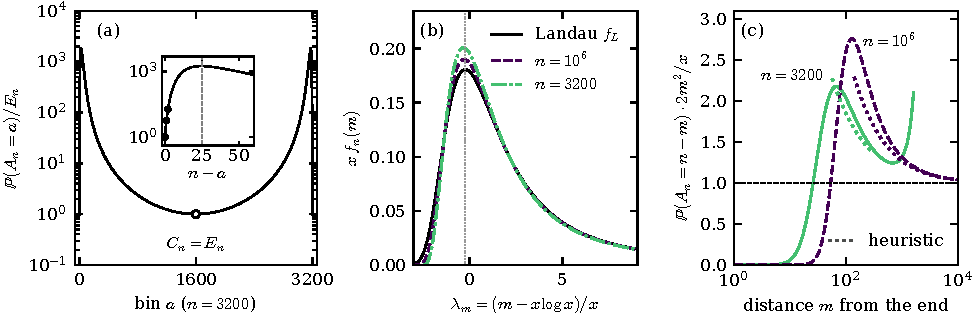
\includegraphics[width=\textwidth]{figures/shape}
\caption{The elephant walk at its crossing. (a) The law of $A_n$ at
$n=3200$ and its crossing $x=11.5468$, divided by the end $E_n$. The center
equals the end, and the law rises from each end to a mode and falls to the
center. The inset shows the last 60 bins, with dots at bins $n$, $n-1$ and
$n-2$. The end is below its neighbor, and the modes are 25 steps from each end
(dashed). (b) The law of $M_n$, scaled as $xf_n(m)$, against
$\lambda_m=(m-x\log x)/x$, with the Landau density $f_L$. The dotted line is
its mode $\lambda_0$. (c) The tail $\Prob(A_n=n-m)$ divided by $x/(2m^2)$. The
dashed line is the limit 1 of Theorem~\ref{thm:profile}, and the dotted
curves are the heuristic correction $1+x(2\log m+2\gamma-3)/m$ for
$2x\log x\le m\le n/x$. The rise of the $n=3200$ curve near $m=n/2$ is the
mirror term $f_n(n-m)$. At $n=10^6$ we use $x=g_n=22.4407$.}
\label{fig:shape}
\end{figure}

\subsection{The bulk}

Let $\CP_n$ be the law of $\sum_{d=1}^{n-1}dN_d$, where the $N_d$ are
independent Poisson variables with means $x/(d(d+1))$. On average
$x/(d(d+1))$ flipped vertices have a family of size $d$. If no 2 flips fall in
the same family, which is likely when $x^2\log n/n$ is small, then $M_n$ is the
total size of the flipped families, and this is close to a compound Poisson
sum.

\begin{remark}[compound Poisson and Landau limits, proofs omitted]\label{rem:bulk}
For $n\ge2$ and $0<\varepsilon\le\frac14$, Fourier inversion, the tree of
Lemma~\ref{lem:tree} and the Efron--Stein inequality~\cite{efronstein1981}
give
$\sup_m\lvert f_n(m)-\CP_n(m)\rvert\le\delta_B:=\frac{x^2\log n}{n}
+\frac{4x^2}{n}e^{4x^2/n}+\frac{4x^2(H_n^2+H_n)}{n}$. Let $f_L$ be the Landau
density, with $\int e^{-u\lambda}f_L(\lambda)\,d\lambda=u^u$ for $u>0$, and put
$\lambda_m=(m-x\log x)/x$. Families of size $d$ are flipped at rate about
$x/d^2$, so the families of size up to about $x$ add up to nearly $x\log x$,
and the few families of size of order $x$ give fluctuations of order $x$.
Under the standing assumptions of this section, comparing characteristic
functions then gives $\sup_m\lvert xf_n(m)-f_L(\lambda_m)\rvert\le
C(\frac{1+\log x}x+\frac xn)+x\delta_B$ with an absolute constant $C$. So
$(M_n-x\log x)/x$ tends to the Landau law when $x\to\infty$ and
$x^3\log^2n/n\to0$, in particular at the crossing. We omit the details of
these 2 bounds. At $n=10^6$ and $x=22.4407$ the bound $\delta_B$ is still about
$0.46$, but there $\lvert f_n(m)/\CP_n(m)-1\rvert\le3.5\cdot10^{-4}$ for
$1\le m\le10^4$. At every tested crossing $m^*$ equals the mode of $\CP_n$. If
$f_L''(\lambda_0)<0$ at the mode $\lambda_0=-0.2228$ of $f_L$, then the
unimodality of $f_L$~\cite{yamazato1978} and the bound above give
$m^*=x\log x+\lambda_0x+O(\sqrt{x\log x})$ at the crossing for large $n$. We
computed $f_L''(\lambda_0)=-0.0789$ by quadrature but did not certify its
sign.
\end{remark}

\subsection{The tail}

\begin{theorem}[the tail]\label{thm:profile}
Let $n$ be even, and let $x=n\varepsilon\ge1$ depend on $n$ with
$x\log^2n/n\to0$. Let $\omega_n\to\infty$ with $\omega_nx\log^2(x+1)=o(n)$, and
let $\delta'_n\to0$. Then
\[
 f_n(m)=\frac{x}{m(m+1)}\bigl(1+o(1)\bigr)\qquad\text{and}\qquad
 \Prob(A_n=n-m)=\frac{x}{2m^2}\bigl(1+o(1)\bigr),
\]
uniformly for $\omega_nx\log^2(x+1)\le m\le\delta'_nn$.
\end{theorem}

In the proof (Appendix~\ref{app:shape}) the lower bound uses the first flipped
family, which has size $m$ with probability about $x/(m(m+1))$ by
Lemma~\ref{lem:B-D}, while the other flips change the count only by a relative
amount of order $x\log m/m$. For the upper bound we show $\Prob(M_n\ge
m)\le\frac xm(1+O(x\log^2m/m))$, and the unimodality of $f_n$ turns this into a
local bound. The mirror term $f_n(n-m)$ is at most $C_n=O(x/n^2)$ by
Lemma~\ref{lem:unimodal} and Theorem~\ref{thm:erw-bounds}(b), so bin $n-m$ is
reached through a family of size $m$ only when $X_1=+1$, and this gives the
constant $\frac12$. At $n=10^6$, $x=22.4407$ and $m=10^4$ the exact ratio
$\Prob(A_n=n-m)/(x/m^2)$ is $0.51889$. At moderate $m$, $\CP_n$ suggests $f_n(m)\,m(m+1)/x\approx1+x(2\log m+2\gamma-3)/m$, and
this factor is still about $2$ near $m=70$ when $n=1600$.

\subsection{The center}

\begin{theorem}[shape at the crossing]\label{thm:shape}
There are absolute constants $C_{\rm w}$ and $n_0$ with the following
property. Let $n\ge n_0$ be even with $x_n\in[2,n^{1/4}]$. Then at the
crossing $\Prob(A_n=a)>C_n$ for every $1\le a\le n-1$ with
$\lvert a-h\rvert\ge C_{\rm w}(nx_n\log n)^{1/2}$.
\end{theorem}

By Theorem~\ref{thm:erw-crossing}, $x_n\in[2,n^{1/4}]$ for large $n$, so at the
crossing the window has width of order $n^{1/2}\log n$.

\begin{proof}
Write $x=x_n$ and $\varepsilon=\varepsilon_n$, so that $C_n=E_n$. By
symmetry we take $a=n-m$ with $1\le m\le h$, and put $t=h-m$. Since $2\le
x\le n^{1/4}$, every error term below is bounded by a function of $n$ alone,
and we take $n$ large. Put
$\Pi(m)=\frac12\bigl[\frac1{m(m+1)}+\frac1{(n-m)(n-m+1)}\bigr]$, so that
$x\Pi(h)=\frac{4\varepsilon}{n+2}$. As $\varepsilon(1+\log n)\to0$,
Theorem~\ref{thm:erw-bounds}(b) gives $C_n\le x\Pi(h)(1+\eta)$ with
$\eta=n^{2\varepsilon}e^{5200\varepsilon}-1$. Put $u=\varepsilon(2\log n+5200)$.
Then $u\le\frac12$ for large $n$, and $e^u-1\le2u$ for $0\le u\le\frac12$, so
$\eta\le2u\le10^4\varepsilon\log n$.

If $m\le m_h$, then $f_n(m)\ge f_n(1)$ by Lemma~\ref{lem:unimodal}. The proof
of Theorem~\ref{thm:dip} gives $f_n(1)\ge\frac x{2(1-\varepsilon)}f_n(0)$, and
$f_n(0)=2E_n=2C_n$. So $\Prob(A_n=n-m)\ge\frac12f_n(m)\ge\frac
x{2(1-\varepsilon)}C_n>C_n$.

If $m_h<m\le n/8$, then $f_n(m)\ge f_n(k)$ with $k=\lfloor n/8\rfloor$, by
Lemma~\ref{lem:unimodal}. Proposition~\ref{thm:B-local-lower}(a) at $k$ gives
$f_n(k)\ge\frac{x}{k(k+1)}(1-O(\frac{x\log n}n))$. So
$\Prob(A_n=n-m)\ge\frac{32x}{n(n+8)}(1-o(1))$, which exceeds
$\frac{4x}{n(n+2)}(1+\eta)\ge C_n$.

If $n/8<m\le h$, then $m$ and $n-m$ are at least $n/8$, and
Proposition~\ref{thm:B-local-lower} at $m$ and at $n-m$ gives
$\Prob(A_n=n-m)\ge x\Pi(m)(1-\bar e)$ with $\bar e=O(x\log n/n)$. Put $N=n+1$
and $s=2t/N$, so that $m+\frac12=\frac N2(1-s)$ and $n-m+\frac12=\frac
N2(1+s)$. Since $\frac1{k(k+1)}\ge(k+\frac12)^{-2}$ and
$\Pi(h)=\frac1{h(h+1)}=(\frac N2)^{-2}(1-N^{-2})^{-1}$, we get
$\frac{\Pi(m)}{\Pi(h)}\ge\frac12[(1-s)^{-2}+(1+s)^{-2}](1-N^{-2})\ge(1+3s^2)(1-N^{-2})$,
because $\frac12[(1-s)^{-2}+(1+s)^{-2}]=\sum_{k\ge0}(2k+1)s^{2k}$. With $b=\bar
e+N^{-2}\le\frac12$ this gives $\Prob(A_n=n-m)\ge x\Pi(h)(1+3s^2)(1-b)\ge
x\Pi(h)(1+\frac32s^2-b)$, which exceeds $x\Pi(h)(1+\eta)\ge C_n$ as soon as
$\frac32s^2>\eta+b$. Now $\eta+b\le A_2x\log n/n$ for an absolute constant
$A_2$, since $x\ge2$, and $s\ge t/n$. So the condition holds when $t\ge C_{\rm
w}(nx\log n)^{1/2}$ with $C_{\rm w}^2>2A_2/3$.
\end{proof}

The window has this size because, at distance $t$ from $h$, the main term
$x\Pi(m)$ exceeds its value at $h$ by a factor of about $1+12t^2/n^2$, while we
know $C_n$ and the law only up to relative errors of order $x\log n/n$. We did
not compute $C_{\rm w}$ or $n_0$. Inside the window the proof gives nothing,
and closing it needs second differences of the law.

\begin{conjecture}[convexity between the humps]\label{conj:convex}
For every $n\ge10$ and $x=x_n$, the second difference
$\Prob(A_n=a-1)-2\Prob(A_n=a)+\Prob(A_n=a+1)$ is positive for
$2m^*+1\le a\le n-2m^*-1$.
\end{conjecture}

With the symmetry of the law, the conjecture makes the law strictly convex on
$[2m^*,n-2m^*]$, so $h$ is its unique minimizer there (the 2 central bins for
odd $n$). The next corollary shows that $m^*=o(n)$ at the crossing.

\begin{corollary}[the modes]\label{cor:modes}
For large even $n$ the modes $a^*$ of the law of $A_n$ at the crossing
satisfy $\min(a^*,n-a^*)=O(x_n\log^2x_n)$.
\end{corollary}

\begin{proof}
Write $x=x_n$ and $\varepsilon=\varepsilon_n$. By
Theorem~\ref{thm:erw-crossing}, $x\sim2\log n$, so for large $n$ the
hypotheses of Theorem~\ref{thm:erw-bounds}(b) and Lemma~\ref{lem:B-mode}
hold. The law is symmetric about $h$, so $m^*=\min(a^*,n-a^*)$ maximizes
$f_n(m)+f_n(n-m)$ over $0\le m\le h$. Lemma~\ref{lem:B-mode} gives $m_h\le h$
for large $n$. So Lemma~\ref{lem:unimodal} and
Theorem~\ref{thm:erw-bounds}(b) give $f_n(n-m)\le f_n(h)=C_n=O(x/n^2)$ for
$m\le h$, and hence $f_n(m^*)\ge f_n(m_h)-C_n$. Let $\ell$ be as in the proof
of Lemma~\ref{lem:B-mode}. Then $f_n(m_h)\ge f_n(\ell)\ge\frac
x{2\ell(\ell+1)}$, so $f_n(m^*)\ge\frac x{4\ell(\ell+1)}$ for large $n$. If
$m^*>m'=\max(m_h,\ell)$, then Lemmas~\ref{lem:B-sandwich}
and~\ref{lem:B-tail} give $(m^*-m'+1)f_n(m^*)\le\Prob(M_n\ge\ell)\le
xH_\ell/\ell$. Hence $m^*\le\max(m_h,\ell)+4(\ell+1)H_\ell$ in every case.
Finally Lemma~\ref{lem:B-mode} gives $m_h=O(x\log^2x)$, and $\ell=O(x\log x)$
and $H_\ell=O(\log x)$.
\end{proof}

So for large even $n$ Theorem~\ref{thm:shape} covers the bins outside
$[2m^*,n-2m^*]$, and the conjecture would make the center the unique interior
minimum. The conjecture holds for every $10\le n\le600$ and for
$n=800,1600,\dots,25600$. On the closed range
$[2m^*,n-2m^*]$ it fails only at the 2 endpoints and only for some $n\le51$.
Heuristically, a concave stretch of $f_n$ far from its mode is added to the
tail $x/(2r^2)$ of the other branch, with $r=n-a$, and the second difference
$3x/r^4$ of this tail beats the concave curvature, which is of order
$x^2/(n^2r^3)$. We leave open the
window around the center, the tail between $x\log x$ and $x\log^2x$, and
effective constants in Theorems~\ref{thm:profile} and~\ref{thm:shape}.

\section{Heavy-tailed runs}\label{sec:heavy}

In this section the walk remembers the time since its last switch. The steps form
maximal runs whose directions alternate. The first run has length $D$, and the later
runs have i.i.d.\ lengths $\xi_1,\xi_2,\dots$ distributed as $\xi$, where
$\bar F(k)=\Prob(\xi\ge k)=k^{-\alpha}$ for $k\ge1$ and some $\alpha>0$. So
$p_k=\Prob(\xi=k)=k^{-\alpha}-(k+1)^{-\alpha}>0$ for every $k\ge1$. The first direction
is fair, and $D$, $(\xi_i)$ and the first direction are independent. With a fresh start
$D$ has the law of $\xi$. For $\alpha>1$ the stationary start is
$\Prob(D=d)=\bar F(d)/\mu$, where $\mu=\E\xi=\zeta(\alpha)$. This law is stationary,
since the number of steps left in the current run (counting the current one) is a Markov
chain that moves from $k\ge2$ to $k-1$ and from $1$ to a fresh copy of $\xi$, and
$\bar F(k)=\bar F(k+1)+p_k\bar F(1)$ makes $\bar F(k)/\mu$ invariant. We define $A_n$,
$C_n$ and $E_n$ as in Section~\ref{sec:intro}, put $R_n=E_n/C_n$, and write $\Prob_+$
for the law given that the first run is $+$.

\begin{proposition}[the edge]\label{prop:edge}
For every law of $D$, $E_n=\frac12\Prob(D\ge n)$. With a fresh start
$E_n=\frac12n^{-\alpha}$. With the stationary start
$E_n=\zeta(\alpha,n)/(2\zeta(\alpha))=n^{1-\alpha}(1+\theta_n(\alpha-1)/n)/(2(\alpha-1)\zeta(\alpha))$
for some $\theta_n\in[0,1]$, where $\zeta(\alpha,n)=\sum_{k\ge n}k^{-\alpha}$ is the
Hurwitz zeta function.
\end{proposition}

\begin{proof}
All $n$ steps are $+1$ exactly when the first direction is $+$ and $D\ge n$. Hence
$E_n=\frac12\Prob(D\ge n)$, and $\Prob(\xi\ge n)=n^{-\alpha}$. For the stationary start
$\Prob(D\ge n)=\zeta(\alpha,n)/\zeta(\alpha)$. Since $x^{-\alpha}$ is decreasing,
$\int_n^\infty x^{-\alpha}dx\le\zeta(\alpha,n)\le n^{-\alpha}+\int_n^\infty x^{-\alpha}dx$,
and the integral equals $n^{1-\alpha}/(\alpha-1)$.
\end{proof}

So the edge only sees the first run, while the center depends on all the runs. Let
$\tau_m=\xi_1+\dots+\xi_m$ with $\tau_0=0$, $u_m(k)=\Prob(\tau_m=k)$ and
$q_m(k)=\Prob(\tau_{m-1}<k\le\tau_m)=\sum_{j\ge1}\bar F(j)u_{m-1}(k-j)$ for $m,k\ge1$.
For the delayed versions let $D$ be independent of $(\xi_i)$, and put
$u^D_m(k)=\Prob(D+\tau_{m-1}=k)$, $q^D_1(k)=\Prob(D\ge k)$ and
$q^D_m(k)=\Prob(D+\tau_{m-2}<k\le D+\tau_{m-1})$ for $m\ge2$. For the stationary start
$u^D_m(k)=\sum_d\frac{\bar F(d)}{\mu}u_{m-1}(k-d)=q_m(k)/\mu$.

The $+$ runs and the $-$ runs form 2 independent renewal processes. The walk is in bin
$a$ at time $n$ exactly when one of them sits at its level and the other is inside a run
that covers its level.

\begin{proposition}[two renewal processes]\label{prop:tworenewal}
Let $D$ have any law on $\{1,2,\dots\}$. For $a+b=n$ with $a,b\ge1$,
\[
 \Prob_+(A_n=a)=\sum_{m\ge1}\Bigl[u_m(b)\,q^D_{m+1}(a)+u^D_m(a)\,q_m(b)\Bigr],
\]
and $\Prob_+(A_n=n)=\Prob(D\ge n)$. In particular, for even $n$,
$C_n=\sum_{m\ge1}[u_m(h)q^D_{m+1}(h)+u^D_m(h)q_m(h)]$. For the fresh start this is
$C_n=\sum_mu_m(h)[q_m(h)+q_{m+1}(h)]$.
\end{proposition}

\begin{proof}
Let the $+$ runs have lengths $D,\xi^+_2,\xi^+_3,\dots$ and the $-$ runs
$\xi^-_1,\xi^-_2,\dots$, and let $s^\pm_j$ be the sum of the first $j$ lengths of each
sign, with $s^\pm_0=0$. So $s^+_j$ has law $u^D_j$ and $s^-_j$ has law $u_j$, and the 2
sequences are independent. The $j$-th $+$ run covers the steps in
$(s^+_{j-1}+s^-_{j-1},\,s^+_j+s^-_{j-1}]$, and the $j$-th $-$ run covers
$(s^+_j+s^-_{j-1},\,s^+_j+s^-_j]$. If step $n=a+b$ is in the first run then $A_n=n$,
which happens exactly when $D\ge n$. If it is in the $j$-th $+$ run with $j\ge2$, then
$A_n=n-s^-_{j-1}$, so $A_n=a$ means $s^-_{j-1}=b$ and $s^+_{j-1}<a\le s^+_j$, which has
probability $u_{j-1}(b)q^D_j(a)$. If it is in the $j$-th $-$ run, then $A_n=s^+_j$, so
$A_n=a$ means $s^+_j=a$ and $s^-_{j-1}<b\le s^-_j$, which has probability
$u^D_j(a)q_j(b)$. Summing over these disjoint cases, with $m=j-1$ in the first and $m=j$
in the second, gives the formula. For even $n$ the symmetry gives
$C_n=\frac12[\Prob_+(A_n=h)+\Prob_+(A_n=n-h)]=\Prob_+(A_n=h)$.
\end{proof}

This identity is the coefficient form of the double transform of Godr\`eche and
Luck~\cite[Section~7]{godrecheluck2001} for the occupation time of an alternating
renewal process.

\begin{lemma}[stable and local limits]\label{lem:stable}
Let $1<\alpha<2$ and $a_m=m^{1/\alpha}$. Put
$K_\alpha=\Gamma(2-\alpha)/(\alpha-1)=-\Gamma(1-\alpha)>0$ and
$\sigma_\alpha=2K_\alpha\lvert\cos\frac{\pi\alpha}2\rvert$.
\begin{enumerate}[(i)]
\item $\E e^{i\theta\xi}=1+i\mu\theta+K_\alpha(-i\theta)^\alpha+O(\theta^2)$ as
$\theta\to0$, with the principal branch.
\item $(\tau_m-m\mu)/a_m$ converges in law to a variable $G$ with
$\E e^{-sG}=e^{K_\alpha s^\alpha}$ for $s\ge0$ and
$\E e^{i\theta G}=\exp(K_\alpha(-i\theta)^\alpha)$. The law of $G$ is totally skewed to
the right and has a bounded, uniformly continuous density $g$ with $g(z)\to0$ as
$\lvert z\rvert\to\infty$.
\item (Gnedenko) $\sup_k\lvert a_mu_m(k)-g((k-m\mu)/a_m)\rvert\to0$, and
$\bar u:=\sup_{m\ge1}\sup_ka_mu_m(k)<\infty$.
\item If $G'$ is an independent copy of $G$, then $G-G'$ is symmetric $\alpha$-stable
with $\E e^{i\theta(G-G')}=e^{-\sigma_\alpha\lvert \theta\rvert^\alpha}$, and
$I_\alpha:=\int_{\mathbb R}g(z)^2\,dz=\Gamma(1+1/\alpha)/(\pi\sigma_\alpha^{1/\alpha})$.
\end{enumerate}
\end{lemma}

\begin{proof}
(i) Summation by parts gives $1-\E x^\xi=(1-x)\sum_{k\ge1}\bar F(k)x^{k-1}$ for
$\lvert x\rvert\le1$. With $x=e^{-u}$ and
$\mathrm{Li}_\alpha(w)=\sum_{k\ge1}k^{-\alpha}w^k$ this is
$1-\E e^{-u\xi}=(e^u-1)\mathrm{Li}_\alpha(e^{-u})$. For $\operatorname{Re}u\ge0$ and
$0<\lvert u\rvert<2\pi$, \cite[25.12.12]{dlmf} gives
$\mathrm{Li}_\alpha(e^{-u})=\Gamma(1-\alpha)u^{\alpha-1}+\zeta(\alpha)+O(\lvert u\rvert)$.
So $1-\E e^{-u\xi}=\mu u+\Gamma(1-\alpha)u^\alpha+O(\lvert u\rvert^2)$, and $u=-i\theta$
gives (i). (ii) By (i),
$e^{-i\mu t}\E e^{it\xi}=1+K_\alpha(-i\theta)^\alpha/m+O(\theta^2m^{-2/\alpha})$ for
$t=\theta/a_m$. As $2/\alpha>1$, the characteristic function of $(\tau_m-m\mu)/a_m$
tends to $\exp(K_\alpha(-i\theta)^\alpha)$, whose modulus
$\exp(-\frac12\sigma_\alpha\lvert\theta\rvert^\alpha)$ is integrable. L\'evy's
continuity theorem, Fourier inversion and the Riemann--Lebesgue lemma give $G$ and $g$
(the domain of attraction also follows from \cite[Theorem~XVII.5.2]{feller1971}). For
real $s>0$, the expansion of $1-\E e^{-u\xi}$ above with $u=s/a_m$ gives
$\E e^{-s(\tau_m-m\mu)/a_m}\to e^{K_\alpha s^\alpha}$ in the same way,
and with $2s$ in place of $s$ this gives uniform integrability, so
$\E e^{-sG}=e^{K_\alpha s^\alpha}$. (iii) Every $p_k$ is positive, so $\xi$ has maximal
span 1, and Gnedenko's local limit theorem~\cite[Chapter~4]{ibragimovlinnik1971}
gives the limit. Then
$a_mu_m(k)\le\lVert g\rVert_\infty+1$ for large $m$ and $a_mu_m(k)\le a_m$ for the
others, so $\bar u<\infty$. (iv) The function
$\lvert\E e^{i\theta G}\rvert^2=e^{-\sigma_\alpha\lvert\theta\rvert^\alpha}$ is the
characteristic function of $G-G'$, and Plancherel's theorem gives
$I_\alpha=\frac1{2\pi}\int e^{-\sigma_\alpha\lvert\theta\rvert^\alpha}d\theta$, which is
$\Gamma(1+1/\alpha)/(\pi\sigma_\alpha^{1/\alpha})$.
\end{proof}

\begin{theorem}[the center for $1<\alpha<2$]\label{thm:center}
Let $1<\alpha<2$ and let $D$ be any a.s.\ finite first run, in particular either start.
As $n\to\infty$ over even $n$,
\[
 C_n\sim2I_\alpha\Bigl(\frac{\mu}{h}\Bigr)^{1/\alpha}
 =\frac{2\Gamma(1+1/\alpha)}{\pi}\Bigl(\frac{\mu}{K_\alpha\lvert\cos(\pi
 \alpha/2)\rvert\,n}\Bigr)^{1/\alpha}.
\]
\end{theorem}

Both kinds of runs must fill about $h$ steps, which takes about $h/\mu$ runs of each
kind. Each renewal process is then within about $n^{1/\alpha}$ of its mean, so the 2
meet at a given level with probability of order $n^{-1/\alpha}$. In the proof (Appendix~\ref{app:heavy}) we split
the sum in Proposition~\ref{prop:tworenewal} by the number $m$ of runs. With
$b_h=(h/\mu)^{1/\alpha}$, the terms with $\lvert m\mu-h\rvert\le Mb_h$ form a Riemann
sum for $2b_h^{-1}\int_{-M}^Mg^2$ by Lemma~\ref{lem:stable}(iii). The terms with
$m\le h/(4\mu)$ add up to $O(h^{-\alpha})=o(b_h^{-1})$, since a large sum of few runs is
most likely made by one long run. The others add up to
$O(b_h^{-1})\Prob(\lvert G\rvert\ge M-1)+o(b_h^{-1})$, and we let $M\to\infty$.

With a stationary start the first run covers all $n$ steps with probability of order
$n^{1-\alpha}$, and this is comparable with $C_n$ when $1-\alpha=-1/\alpha$, that is
$\alpha^2-\alpha-1=0$.

\begin{corollary}[the golden-ratio exponent]\label{cor:golden}
Let $1<\alpha<2$ and $e(\alpha)=1-\alpha+1/\alpha$. If
$\Prob(D\ge n)\sim c_Dn^{-\beta_D}$ with $c_D,\beta_D>0$, then
$R_n\sim c_Dn^{1/\alpha-\beta_D}/(4I_\alpha(2\mu)^{1/\alpha})$. In particular
$R_n\sim C(\alpha)n^{e(\alpha)}$ for the stationary start and
$R_n\sim C_{\rm fr}(\alpha)n^{e(\alpha)-1}$ for the fresh start, where
\[
 C(\alpha)=\frac{\pi\bigl(K_\alpha\lvert\cos\frac{\pi\alpha}2\rvert
 \bigr)^{1/\alpha}}{4(\alpha-1)\Gamma(1+\frac1\alpha)\,
 \zeta(\alpha)^{1+1/\alpha}},\qquad
 C_{\rm fr}(\alpha)=(\alpha-1)\zeta(\alpha)\,C(\alpha).
\]
Since $e(\alpha)>0$ exactly when $\alpha<\varphi$, with a stationary start the ends win
for all large $n$ if $\alpha<\varphi$, and the center wins if $\alpha>\varphi$. At
$\alpha=\varphi$,
\[
 R_n\to C(\varphi)=\frac{\pi\varphi\bigl(\varphi\,\Gamma(\varphi^{-2})\lvert
 \cos\frac{\pi\varphi}2\rvert\bigr)^{1/\varphi}}{4\,\Gamma(\varphi)\,
 \zeta(\varphi)^{\varphi}}=0.7761317206\ldots,
\]
so the center still wins by the factor $1/C(\varphi)=1.2884$. With a fresh start
$e(\alpha)-1<0$, and the center wins for every $1<\alpha<2$.
\end{corollary}

\begin{proof}
By Proposition~\ref{prop:edge} and Theorem~\ref{thm:center}, with $h=n/2$, we have
$R_n=\Prob(D\ge n)/(2C_n)$, and this is asymptotic to
$c_Dn^{-\beta_D}/(4I_\alpha(2\mu/n)^{1/\alpha})$, which is the general formula. By
Lemma~\ref{lem:stable}(iv),
$4I_\alpha(2\mu)^{1/\alpha}=4\Gamma(1+\frac1\alpha)\mu^{1/\alpha}/(\pi(K_\alpha\lvert\cos\frac{\pi\alpha}2\rvert)^{1/\alpha})$.
The fresh start has $c_D=1$ and $\beta_D=\alpha$, which gives $C_{\rm fr}(\alpha)$. By
Proposition~\ref{prop:edge} the stationary start has $c_D=1/((\alpha-1)\mu)$ and
$\beta_D=\alpha-1$, which gives $C(\alpha)$. Next,
$e(\alpha)=-(\alpha^2-\alpha-1)/\alpha$, and $\varphi$ is the positive root of
$\alpha^2-\alpha-1$. At $\alpha=\varphi$ we have $\alpha-1=1/\varphi$,
$1+1/\alpha=\varphi$ and $2-\alpha=\varphi^{-2}$. So
$K_\varphi=\varphi\,\Gamma(\varphi^{-2})$, and substituting these into $C(\alpha)$ gives
the closed form.
\end{proof}

Corollary~\ref{cor:golden} is the lattice form, with its constant, of the heuristic of
Wang, Li and H\"anggi~\cite[Section~2.1]{wlh2016}. The golden ratio also appears for
the elephant walk, as the log-concavity threshold $1/\varphi$
of~\cite[Proposition~2.2]{glrs2025}, but we know of no connection between the 2. The
approach to $C(\varphi)$ is slow. At $\alpha=\varphi$ we have $R_{10^5}/C(\varphi)=0.938$,
and $R_n$ increases on the computed grid
(Table~\ref{tab:heavy} and Figure~\ref{fig:heavy}).

\begin{table}[t]
\centering\small
\setlength{\tabcolsep}{5pt}
\begin{tabular}{@{}lrlllll@{}}
\toprule
$\alpha$ & $e(\alpha)$ & $C(\alpha)$ & $C_{\rm fr}(\alpha)$ & $R_{1600}$ & $R_{10^4}$ & $R_{10^5}$\\
\midrule
$1.3$ & $+0.469231$ & $0.422717$ & $0.498631$ & $17.7593$ $[1.3180]$ & $38.7537$ $[1.2171]$ & $106.149$ $[1.1317]$\\
$1.5$ & $+0.166667$ & $0.647971$ & $0.846371$ & $2.14409$ $[0.9675]$ & $2.9528$ $[0.9818]$ & $4.37642$ $[0.9914]$\\
$\varphi$ & $0$ & $0.776132$ & $1.073675$ & $0.661763$ $[0.8526]$ & $0.697331$ $[0.8985]$ & $0.727689$ $[0.9376]$\\
$5/3$ & $-1/15$ & $0.835101$ & $1.182237$ & $0.411815$ $[0.8064]$ & $0.389307$ $[0.8614]$ & $0.352822$ $[0.9102]$\\
$1.7$ & $-0.111765$ & $0.880046$ & $1.265508$ & $0.298369$ $[0.7733]$ & $0.262005$ $[0.8334]$ & $0.215839$ $[0.8881]$\\
$1.9$ & $-0.373684$ & $1.438986$ & $2.266075$ & $0.0449706$ $[0.4923]$ & $0.0256505$ $[0.5569]$ & $0.0121612$ $[0.6242]$\\
\bottomrule
\end{tabular}
\caption{Constants of Corollary~\ref{cor:golden} and exact values of $R_n=E_n/C_n$ for
the stationary start, with $R_n/(C(\alpha)n^{e(\alpha)})$ in brackets.}
\label{tab:heavy}
\end{table}

\begin{figure}[t]
\centering
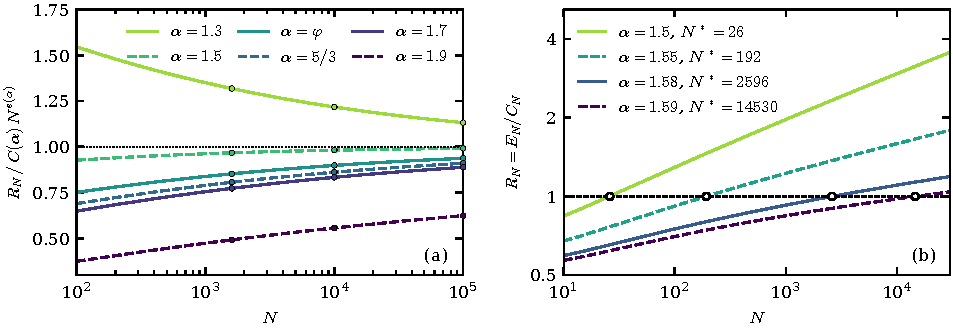
\includegraphics{figures/heavy}
\caption{Alternating runs with a stationary start. (a) $R_n/(C(\alpha)n^{e(\alpha)})$ for
even $n$ from 100 to $10^5$, with the entries of Table~\ref{tab:heavy} as dots. (b)
$R_n$ for $\alpha=1.5,1.55,1.58,1.59$ below $\varphi$. Each curve crosses 1 once on
$10\le n\le3\cdot10^4$, at $n^*(\alpha)$ (circles).}
\label{fig:heavy}
\end{figure}

\begin{table}[t]
\centering\small
\setlength{\tabcolsep}{4pt}
\begin{tabular}{@{}lllll@{}}
\toprule
$\alpha$ & start & center $C_n$ & ratio $R_n$ & status\\
\midrule
$\alpha>2$ & stationary & $\sim\sqrt{2\mu/(\pi vn)}$ & $\sim C_2(\alpha)n^{3/2-\alpha}$ & same argument, omitted\\
$\alpha=2$ & stationary & $\sim\sqrt{2\mu/(\pi n\log n)}$ & $\sim\sqrt{\pi\log n/(8\zeta(2)^3n)}$ & same argument, omitted\\
$1<\alpha<2$ & fresh & $\sim2I_\alpha(\mu/h)^{1/\alpha}$ & $\sim C_{\rm fr}(\alpha)n^{e(\alpha)-1}\to0$ & Corollary~\ref{cor:golden}\\
$\alpha=1$ & fresh & $\approx2/(\pi^2\tilde m_h)$ & $\approx\pi^2\tilde m_h/(8h)\sim\pi^2/(8\log n)$ & heuristic\\
$0<\alpha<1$ & fresh & $\sim\frac2\pi\tan\frac{\pi\alpha}2\cdot\frac1n$ & $\sim\frac{\pi}{4\tan(\pi\alpha/2)}\,n^{1-\alpha}\to\infty$ & proof omitted\\
\bottomrule
\end{tabular}
\caption{Outcomes of Remark~\ref{rem:other}. The center wins when $R_n\to0$ and the ends
win when $R_n\to\infty$.}
\label{tab:outcomes}
\end{table}

\begin{remark}[other exponents]\label{rem:other}
Table~\ref{tab:outcomes} collects the cases that Corollary~\ref{cor:golden} leaves out.
For $\alpha>2$ let $v=\Var\xi=2\zeta(\alpha-1)-\zeta(\alpha)-\zeta(\alpha)^2$ and
$C_2(\alpha)=\sqrt{\pi v/(2\mu)}/(2(\alpha-1)\mu)$. The proof of
Theorem~\ref{thm:center} works with the Gaussian local limit theorem and
$a_m=\sqrt{vm}$, and for $\alpha=2$ with the norming $a_m\sim\sqrt{m\log m}$
of~\cite[Theorem~XVII.5.3 and eq.~(XVII.5.23)]{feller1971}. In these 2 rows the center
formula holds for every a.s.\ finite first run, so a fresh start also gives $R_n\to0$.
For $\alpha=1$ the same proof with a skewed Cauchy limit and the centering
$m(H_{m+1}-1)$ suggests the row of the table, where $\tilde m_h$ solves
$m(H_{m+1}-1)=h$. For $0<\alpha<1$ only the fresh start makes
sense, and $\frac2\pi\tan\frac{\pi\alpha}2$ is the density at $\frac12$ of Lamperti's
occupation-time law~\cite{lamperti1958,godrecheluck2001}. Here the proof splits the sum
in Proposition~\ref{prop:tworenewal} on the scale of $\log m$ and uses the moments of a
positive stable law~\cite[Theorem~2.6.3]{zolotarev1986} and the series for its
density~\cite[Lemma~XVII.6.1]{feller1971}. We omit the details for $\alpha\ge2$ and
$0<\alpha<1$. So with a fresh start the threshold is $\alpha=1$.
\end{remark}

\begin{remark}[crossover sizes and heat conduction]\label{rem:crossover}
For $\alpha<\varphi$ and a stationary start the crossover is late when $\alpha$ is close
to $\varphi$. For $\alpha=1.5,1.55,1.58,1.59$ and every even $n$ in $[10,3\cdot10^4]$,
$R_n-1$ changes sign once, at $n^*(\alpha)=26,192,2596,14530$. Heuristically, $C(\alpha)n^{e(\alpha)}=1$
gives $\log n^*(\alpha)=0.1834/(\varphi-\alpha)+O(1)$ as $\alpha\uparrow\varphi$. At the
value $\alpha=5/3$ of L\'evy-walk models of heat conduction~\cite{dsd2013,zdk2015},
$R_n\sim C(5/3)n^{-1/15}$ with $C(5/3)=0.8351$.
\end{remark}

\begin{remark}[aging]\label{rem:aging}
Let the walk take a fair first step and then switch direction at step $k\ge2$ with
probability $c/k$, where $0<c<2$. Then $A_n/n$ converges in law to
$\mathrm{Beta}(c,c)$~\cite[Example~1.1 and Theorem~1.4]{ds2007} (their chain is this
walk for $c\le1$), \cite[Theorem~1]{ev2018}, and the limit is uniform exactly when
$c=1$~\cite[Remark~2]{ev2018}. At finite $n$ the first step matters. Let $\Prob_+$ be
the law given that the first step is $+1$, and let $X_n$ be the last step. At $c=1$
induction on $n\ge2$ gives $\Prob_+(A_n=s,\,X_n=+1)=\frac{s-1}{n(n-1)}$ and
$\Prob_+(A_n=s,\,X_n=-1)=\frac{n-s}{n(n-1)}$ for $1\le s\le n$, so $A_n$ is uniform on
$\{1,\dots,n\}$ (after a shift of one step this is the exercise
in~\cite[footnote~1 on p.~6]{evw2020}). Compared with no switch, a switch at time $t$
multiplies the probability of a path by $c/(t-c)$, which increases in $c$, and every
path with $A_n<n$ switches. So by the argument of Proposition~\ref{prop:mlr},
$\Prob_+(A_n=s)/\Prob_+(A_n=n)$ increases strictly in $c$ for $1\le s\le n-1$, and the
fixed-start crossing is exactly $c=1$ for every $n$ and every bin. With a fair first
step the ends are $\frac1{2n}$ at $c=1$ and every interior bin is $\frac1n$. By the same
argument $C_n/E_n$ increases strictly in $c$, from $0$ as $c\downarrow0$ to $2$ at
$c=1$, so the crossing $c_n$ is unique and below $1$. For even $n$,
$c_n=1-\log2/(\log n+\gamma+2-2\log2)+O((\log n)^{-3})$, and the exact
crossing at $n=200$ is $c_{200}=0.8925$, against $0.8932$ from the first 2
terms. This follows from $E_n=\frac12\prod_{k=2}^n(1-c/k)$ and a local limit
theorem with a rate, $nC_n\to4^{1-c}/\mathrm B(c,c)$ uniformly for $c$ near $1$, and we
omit the details. The exact statements here are also proved in Lean
(Section~\ref{sec:verify}).
\end{remark}

We do not know a rate in Theorem~\ref{thm:center}, whether $R_n$ is monotone with a
single sign change of $R_n-1$, how to make the case $\alpha=1$ rigorous, or the full
shape of the law of $A_n$.

\section{Verification}\label{sec:verify}

All computations are in Python, and the main ones were done by 2 independent
methods. For example, a forward recursion for the law of $M_n$ and a backward
recursion for $V_s$ agree to about $10^{-14}$ at $n=12800$. The proofs use
computation in only 3 places. Some constants are values of explicit sums and
integrals, Remark~\ref{rem:bulk} uses a computed sign, and
Corollary~\ref{cor:dip} holds for every even $n\ge8$ but for $n<1688$ its
hypothesis rests on a computation of $C_n/E_n$ at $\varepsilon=2/(n+2)$.
Conjecture~\ref{conj:convex}, the tables, the figures and the numbers quoted
outside the proofs rest on computation alone. Before each new computation we
wrote down a prediction and a condition that would refute it. Of these
predictions 8 failed, and none of them concerns a statement that we call a
theorem. The scripts, their output and the prediction ledgers are in the
Problem 131 folder of \url{https://github.com/apemm/Kagey-Problems}, where
\texttt{SUPPLEMENT.md} says what each script checks and
\texttt{python -B verify\_all.py --paper d} reruns them in a few minutes. The
exact and finite statements, among them Proposition~\ref{prop:mlr},
Lemma~\ref{lem:unimodal}, Theorem~\ref{thm:dip} and the identities behind
Corollary~\ref{cor:golden}, are also proved in Lean~4 in
\texttt{lean/PaperD}, and \texttt{MAP.md} there lists each one with its Lean
name.

\paragraph{Acknowledgment.}
The Lean code for this paper was generated by AI. AI was also used to
revise some of the writing and to help cross-verify the code.


\appendix
\section{Proof of \texorpdfstring{Theorem~\ref{thm:erw-bounds}}{Theorem 2.6}}\label{app:erw}

Throughout, $N\ge2$ is even and we condition on $X_1=+1$. By
Proposition~\ref{prop:first-mutation}(a) we need to bound $V_{t+1}(1)$, and we
compare $V$ with explicit hitting probabilities of P\'olya urns. Let
$\mathcal L_sF(b)=(1-r_s(b))F(b)+r_s(b)F(b+1)$, so that $V_s=\mathcal L_sV_{s+1}$ and $V_N(b)=\mathbf 1\{b=h\}$. Both $M_t$
and $t-M_t\ge1$ are nondecreasing. So from $b\ge1$ the chain stays at states
$\ge1$, and for $b\ge1$ we have $V_s(b)=0$ unless $b$ is feasible, that is,
$b\in\mathcal S_s=\{b\in\Z:1\le b\le h,\ 1\le s-b\le h\}$. Note that
$\mathcal S_N=\{h\}$.

For $c\ge0$ the P\'olya$(c)$ chain moves at time $s$ from $b$ to $b+1$ with
probability $r^c_s(b)=\frac{b+c}{s+2c}$. It is P\'olya's urn with weights
$b+c$ and $s-b+c$ for the 2 colors, that is, with $c$ extra balls of each
color. For $b+c>0$ and $s-b+c>0$ let
$\Phi^c_s(b)=\binom{N-s}{h-b}\mathrm B(h+c,h+c)/\mathrm B(b+c,s-b+c)$, where
$\mathrm B$ is the beta function and the binomial coefficient is 0 unless
$0\le h-b\le N-s$. Theorem~\ref{thm:erw-bounds}(a) will follow from
Lemma~\ref{lem:A-polya}(d), and (b) from Proposition~\ref{prop:A-super}.

\begin{lemma}\label{lem:A-polya}
Let $c\ge0$, $1\le s\le N$, $b+c>0$ and $s-b+c>0$.
\begin{enumerate}[(a)]
\item $\Phi^c_s(b)$ is the probability that the P\'olya$(c)$ chain at $b$ at
time $s$ is at $h$ at time $N$. So $\Phi^c_N(b)=\mathbf 1\{b=h\}$, and
$\Phi^c_s(b)=r^c_s(b)\Phi^c_{s+1}(b+1)+(1-r^c_s(b))\Phi^c_{s+1}(b)$ for
$s<N$.
\item If $s<N$ and $\Phi^c_s(b)>0$, then
$r^c_s(b)\Phi^c_{s+1}(b+1)/\Phi^c_s(b)=\bar r_s(b):=\frac{h-b}{N-s}$.
\item If $0<\varepsilon<\frac12$ and $\beta=\frac{\varepsilon}{1-2\varepsilon}$,
then $r_s(b)=r^{\beta s}_s(b)$ for $0\le b\le s$.
\item If $0<\varepsilon<\frac12$ and $0\le c\le\beta s$, then
$V_s(b)\ge\Phi^c_s(b)$ for $1\le b\le s-1$. In particular
$V_{t+1}(1)\ge\Phi^0_{t+1}(1)=\pi_t$ for $1\le t\le h$.
\end{enumerate}
\end{lemma}

\begin{proof}
(a) Let $x=b+c$, $y=s-b+c$ and $(x)_k=x(x+1)\cdots(x+k-1)$. As in the proof
of Lemma~\ref{lem:urn}, each order of the $N-s$ draws with $h-b$ draws of
the first color has probability
$(x)_{h-b}(y)_{N-s-h+b}/(x+y)_{N-s}=\mathrm B(h+c,h+c)/\mathrm B(x,y)$, and
there are $\binom{N-s}{h-b}$ such orders. The recursion is the Markov
property.

(b) Use $\binom{N-s-1}{h-b-1}/\binom{N-s}{h-b}=\frac{h-b}{N-s}$ and
$\mathrm B(x,y)/\mathrm B(x+1,y)=\frac{x+y}x=1/r^c_s(b)$.

(c) Since $1+2\beta=1/(1-2\varepsilon)$, we have
$\frac{b+\beta s}{s+2\beta s}=(1-2\varepsilon)(\frac bs+\beta)=r_s(b)$.

(d) Let $F_u=\Phi^c_u$ on $\{1,\dots,u-1\}$ for $s\le u\le N$. Then $F_u$
vanishes off $\mathcal S_u$ and $F_N(b)=\mathbf 1\{b=h\}$. By (a) and (c),
$\mathcal L_uF_{u+1}(b)-F_u(b)=(r_u(b)-r^c_u(b))(F_{u+1}(b+1)-F_{u+1}(b))$.
Since $r^c_u(b)=\frac12-(\frac u2-b)/(u+2c)$, this is the product of
$\frac u2-b$, $\frac1{u+2c}-\frac1{u(1+2\beta)}\ge0$ (as $c\le\beta s\le\beta
u$) and $F_{u+1}(b+1)-F_{u+1}(b)$. Let
$b\in\mathcal S_u$. If $b=h$ then $b\ge u/2$ and $F_{u+1}(b+1)=0$. If
$u-b=h$ then $b\le u/2$ and $F_{u+1}(b)=0$. Otherwise
$F_{u+1}(b+1)/F_{u+1}(b)=\frac{(h-b)(u-b+c)}{(h-u+b)(b+c)}$, which is
$\ge1$ exactly when $b\le u/2$ (write $b=\frac u2-d$; the difference of
the 2 sides of the inequality is $2d(h+c)$). So in all 3 cases the first and
last factors have the same sign, and $\mathcal L_uF_{u+1}\ge F_u$ on
$\mathcal S_u$, and Lemma~\ref{lem:A-compare}(b) gives $V_s\ge F_s$.
Finally $\Phi^0_{t+1}(1)=\beta_{t+1}(h)=\pi_t$ by (a) and
Lemma~\ref{lem:urn}.
\end{proof}

\begin{lemma}\label{lem:A-compare}
Let $1\le s_0\le N$, and for $s_0\le s\le N$ let $F_s\ge0$ be a function on
$\{1,\dots,s-1\}$.
\begin{enumerate}[(a)]
\item If $F_N(h)\ge1$ and $\mathcal L_sF_{s+1}\le K_sF_s$ on $\mathcal S_s$
for $s_0\le s<N$, with constants $K_s\ge0$, then
$V_s\le\bigl(\prod_{u=s}^{N-1}K_u\bigr)F_s$ on $\mathcal S_s$.
\item If $F_N(b)\le\mathbf 1\{b=h\}$, each $F_s$ vanishes off $\mathcal S_s$,
and $\mathcal L_sF_{s+1}\ge F_s$ on $\mathcal S_s$ for $s_0\le s<N$, then
$V_s\ge F_s$.
\end{enumerate}
\end{lemma}

\begin{proof}
We use backward induction on $s$, from $V_N(b)=\mathbf 1\{b=h\}$. In (a),
$V_{s+1}$ vanishes at infeasible states and $F_{s+1}\ge0$, so on
$\mathcal S_s$ we get
$V_s=\mathcal L_sV_{s+1}\le\prod_{u>s}K_u\,\mathcal L_sF_{s+1}\le\prod_{u\ge s}K_u\,F_s$.
In (b) we get $V_s\ge\mathcal L_sF_{s+1}\ge F_s$ on $\mathcal S_s$, and
$F_s=0\le V_s$ off $\mathcal S_s$.
\end{proof}

For the upper bound we compare $M$ with an urn that has more extra balls,
and we control the cost of each step through the derivative of $\Phi^\tau_s$
in $\tau$. Let $\psi$ be the digamma function.

\begin{lemma}\label{lem:A-cderiv}
Let $2\le s\le N$, $b\in\mathcal S_s$ and $\tau\ge0$. Put $X=b+\tau$,
$Y=s-b+\tau$, $\Sigma=X+Y$ and $z=(s-2b)^2/\Sigma^2$. Then
\[
 \partial_\tau\log\Phi^\tau_s(b)
 <-\log(1-z)+\frac{1+z}{(1-z)\Sigma}+\frac{2(1+z)}{3\Sigma^2(1-z)^2}.
\]
\end{lemma}

\begin{proof}
Since $\log\mathrm B(x,y)=\log\Gamma(x)+\log\Gamma(y)-\log\Gamma(x+y)$, the
derivative is $2\psi(\Sigma)-\psi(X)-\psi(Y)-2\psi(N+2\tau)+2\psi(h+\tau)$.
For $x>0$, \cite[5.9.15]{dlmf} writes $\log x-\frac1{2x}-\psi(x)$ as
$2\int_0^\infty\frac{t\,dt}{(t^2+x^2)(e^{2\pi t}-1)}$, which lies in
$(0,\frac1{12x^2})$ since $\int_0^\infty\frac{t\,dt}{e^{2\pi t}-1}=\frac1{24}$.
We use this upper bound for $\psi(\Sigma)$ and lower bound for $\psi(X)$ and
$\psi(Y)$. The duplication formula \cite[5.5.5]{dlmf} gives
$2\psi(2y)=\psi(y)+\psi(y+\frac12)+2\log2$, and $\psi$ is increasing, so
$2\psi(N+2\tau)-2\psi(h+\tau)>2\log2$. Hence the derivative is less than
$\log\frac{\Sigma^2}{4XY}+(\frac1{2X}+\frac1{2Y}-\frac1\Sigma)
+\frac1{12}(\frac1{X^2}+\frac1{Y^2})$. Now $4XY=\Sigma^2(1-z)$ and
$X^2+Y^2=\Sigma^2(1+z)/2$, so the 3 terms are $-\log(1-z)$,
$\frac{X^2+Y^2}{2XY\Sigma}=\frac{1+z}{(1-z)\Sigma}$ and
$\frac{X^2+Y^2}{12X^2Y^2}=\frac{2(1+z)}{3\Sigma^2(1-z)^2}$.
\end{proof}

\begin{proposition}\label{prop:A-super}
Let $0<\varepsilon<\frac14$, $\kappa=\frac{2\varepsilon}{1-4\varepsilon}$,
$\kappa_s=\kappa(s+10)$ and $\Sigma_s=s+2\kappa_s$. For $1\le s\le N-1$ and
$b\in\mathcal S_s$ let
$\Delta_s(b)=\mathcal L_s\Phi^{\kappa_{s+1}}_{s+1}(b)\big/\Phi^{\kappa_s}_s(b)$.
\begin{enumerate}[(a)]
\item Let $c=\kappa_s$, $c'=\kappa_{s+1}$, $d=\frac s2-b$, $u=\frac{d}{s+2c'}$,
$v=\frac d{N-s}$ and $\rho=\frac{s+2c'}{s(1+2\beta)}$. Then $|u|<\frac12$
and
\[
 \Delta_s(b)=\mathcal J\,\frac{\Phi^{c'}_s(b)}{\Phi^{c}_s(b)},\qquad
 \mathcal J=1-(\rho-1)\frac{u(u+v)}{\frac14-u^2}.
\]
\item $\log \Delta_s(b)\le\frac{\kappa}{\Sigma_s}+\frac{2\kappa}{3\Sigma_s^2}$.
\item For $1\le t\le h$,
$V_{t+1}(1)\le\pi_t\exp\bigl(\kappa\bigl[H_{N-1}-H_t+\frac2{3t}\bigr]
+\kappa_{t+1}\bigl[\log\frac{(t+1)^2}{4t}+\frac23\bigr]\bigr)$.
\item $C_N\le U_N:=\varepsilon c_1e^{\kappa H_{N-1}}\sum_{t=1}^hw_t
(1-\varepsilon)^{t-1}e^{\kappa\mathcal G(t)}$, where
$\mathcal G(t)=(t+11)\bigl(\log\frac{(t+1)^2}{4t}+\frac23\bigr)-H_t+\frac2{3t}$.
\end{enumerate}
\end{proposition}

The slope $\kappa$ solves $2(\kappa-\beta)/(1+2\beta)=\kappa$, so that in (b)
the gain in $\mathcal J$ cancels the main loss from raising the extra balls
from $c$ to $c'$.

\begin{proof}
(a) Write $r'=r^{c'}_s(b)$, $\bar r=\bar r_s(b)$ and $r=r_s(b)$. By
Lemma~\ref{lem:A-polya}(b) with $c'$, and the recursion in
Lemma~\ref{lem:A-polya}(a), we have
$r'\Phi^{c'}_{s+1}(b+1)=\bar r\,\Phi^{c'}_s(b)$ and
$(1-r')\Phi^{c'}_{s+1}(b)=(1-\bar r)\Phi^{c'}_s(b)$. So the numerator of
$\Delta_s(b)$ divided by $\Phi^{c'}_s(b)$ is
$\frac{(1-r)(1-\bar r)}{1-r'}+\frac{r\bar r}{r'}$. Here $r'=\frac12-u$,
$\bar r=\frac12+v$ and $r=\frac12-\rho u$, since
$\frac12-r=(1-2\varepsilon)\frac ds=\rho u$. Over the denominator
$r'(1-r')=\frac14-u^2$ the numerator is $f(u,v)+f(-u,-v)$ with
$f(u,v)=(\frac12+\rho u)(\frac12-v)(\frac12-u)$, and this equals
$\frac14-\rho u^2-(\rho-1)uv$. Also $|d|\le\frac s2-1$, so $|u|<\frac12$.

(b) \emph{Step 1: the factor $\mathcal J$.} Write $c=\kappa_s$,
$c'=c+\kappa$ and $\Sigma=\Sigma_s$. Since
$c'-\beta s=(\kappa-\beta)s+11\kappa$, the choice of $\kappa$ gives
$\rho-1=\kappa+\nu_s$ with $\nu_s=\frac{22\kappa}{s(1+2\beta)}$. As $u$ and
$v$ have the sign of $d$, $u(u+v)\ge u^2$. So
$\mathcal J\le1-(\kappa+\nu_s)W'$ with $z'=4u^2$ and $W'=\frac{z'}{1-z'}$.
Also $\mathcal J>0$ by (a), since $0<r<1$ and $\bar r$, $1-\bar r$ are not
both 0. So $\log\mathcal J\le-(\kappa+\nu_s)W'$.

\emph{Step 2: the ratio $\Phi^{c'}_s/\Phi^c_s$.} The logarithm
$\log(\Phi^{c'}_s(b)/\Phi^c_s(b))$ is the integral over $\tau\in[c,c']$ of
the derivative in Lemma~\ref{lem:A-cderiv}. Its bound increases in $z$ and
decreases in $\Sigma$, while $z$ decreases and $\Sigma$ increases in $\tau$.
So we may take the bound at $\tau=c$, where $X+Y=\Sigma$, and multiply it by
the length $\kappa$ of the interval. Put
$W=\frac z{1-z}$. Then $\frac1{1-z}=1+W$, $\frac{1+z}{1-z}=1+2W$ and
$-\log(1-z)\le W$, so
\begin{equation}\label{eq:A-logD}
 \log \Delta_s(b)\le\kappa\Bigl[W+\frac{1+2W}\Sigma+\frac{2(1+2W)(1+W)}{3\Sigma^2}\Bigr]
 -(\kappa+\nu_s)W'.
\end{equation}
\emph{Step 3: 3 facts.} (i) $X,Y\ge1+c$, since $b\ge1$ and $s-b\ge1$. So
$XY\ge(1+c)\Sigma/2$ and $1+W=\frac{\Sigma^2}{4XY}\le\frac\Sigma{2(1+c)}$.
(ii) $z'=\lambda z$ with $\lambda=(\frac\Sigma{\Sigma+2\kappa})^2
\ge1-\frac{4\kappa}\Sigma$. So $W-W'=\frac{(1-\lambda)z}{(1-z)(1-\lambda z)}
\le(1-\lambda)W(1+W)\le\frac{2\kappa}{1+c}W$ by (i). As $c\ge11\kappa$, this
gives $W'\ge\frac9{11}W$. (iii) $\Sigma\ge s$ and $1+c>\kappa s$. If $W>0$
then $s\ne2b$, and with $b\ge1$, $s-b\ge1$ this forces $s\ge3$, so
$\Sigma^2\ge3s$.

\emph{Step 4: collect the terms.} By (ii) and (iii),
$\kappa(W-W')\le\frac{2\kappa^2}{1+c}W\le\frac{2\kappa}sW$
and $\frac{2\kappa W}\Sigma\le\frac{2\kappa}sW$. Since
$(1+2W)(1+W)=1+3W+2W^2$, $\kappa$ times the last term in the bracket of
\eqref{eq:A-logD} is
$\frac{2\kappa}{3\Sigma^2}+\frac{2\kappa W}{\Sigma^2}
+\frac{4\kappa W^2}{3\Sigma^2}$. Here
$\frac{2\kappa W}{\Sigma^2}\le\frac{2\kappa}{3s}W$ by (iii), and
$\frac{4\kappa W^2}{3\Sigma^2}\le\frac{4\kappa W(1+W)}{3\Sigma^2}
\le\frac{2\kappa W}{3\Sigma(1+c)}\le\frac{2\kappa}{3s}W$ by (i). With
$-\nu_sW'\le-\frac9{11}\nu_sW$ this gives
\[
 \log \Delta_s(b)\le\frac\kappa\Sigma+\frac{2\kappa}{3\Sigma^2}
 +W\Bigl[\frac{16\kappa}{3s}-\frac{18\kappa}{s(1+2\beta)}\Bigr],
\]
and the bracket is negative because $1+2\beta<2$ for $\varepsilon<\frac14$,
so $18/(1+2\beta)>9>16/3$.

(c) Apply Lemma~\ref{lem:A-compare}(a) with $s_0=t+1$, $F_s=\Phi^{\kappa_s}_s$
and $K_s=\exp(\frac\kappa s+\frac{2\kappa}{3s^2})$. This is allowed, since
$F_N(h)=1$, $F_s>0$ on $\mathcal S_s$, and $\mathcal L_sF_{s+1}=\Delta_sF_s\le
K_sF_s$ on $\mathcal S_s$ by (b) and $\Sigma_s\ge s$. Since $1\in\mathcal S_{t+1}$ and
$\sum_{s>t}s^{-2}\le\frac1t$, we get
$V_{t+1}(1)\le e^{\kappa[H_{N-1}-H_t+2/(3t)]}\,\Phi^{\kappa_{t+1}}_{t+1}(1)$.
Now $\log(\Phi^{\kappa_{t+1}}_{t+1}(1)/\pi_t)$ is the integral over
$\tau\in[0,\kappa_{t+1}]$ of the derivative in Lemma~\ref{lem:A-cderiv}, whose
bound is largest at $\tau=0$. There $X=1$, $Y=t$ and
$\frac1{1-z}=\frac{(t+1)^2}{4t}$, and the bound is
$\log\frac{(t+1)^2}{4t}+\frac{t^2+1}{2t(t+1)}+\frac{t^2+1}{12t^2}
\le\log\frac{(t+1)^2}{4t}+\frac23$.

(d) Insert (c) into Proposition~\ref{prop:first-mutation}(a), and use
$\kappa_{t+1}=\kappa(t+11)$ and $\pi_t=c_1w_t$.
\end{proof}

\begin{proof}[Proof of Theorem~\ref{thm:erw-bounds}]
(a) By Proposition~\ref{prop:first-mutation}(a) and
Lemma~\ref{lem:A-polya}(d),
$C_N\ge\varepsilon c_1\sum_tw_t(1-\varepsilon)^{t-1}$. Now
$(1-\varepsilon)^{t-1}\ge1-(t-1)\varepsilon$ and
$\sum_tw_t(t-1)=2-\frac6{h+2}$ by Proposition~\ref{prop:first-mutation}(c).
So $C_N\ge\varepsilon c_1(1-2\varepsilon)$, and $c_1=\frac4{N+2}$.

(b) \emph{Step 1: the constants.} Let $N\ge64$ and
$\varepsilon(1+\log N)\le\frac1{100}$. Then
$\varepsilon<0.002$ and $\kappa\le2\varepsilon(1+8\varepsilon)\le2.1\varepsilon$.
Since $\log\frac{(t+1)^2}{4t}\ge0$ and $\frac23(t+11)>1+\log t\ge H_t$, we
have $\mathcal G(t)>0$. Since $\frac{(t+1)^2}{4t}\le\frac{t+1}2$,
$\frac23<\log2$ and $H_t\ge\frac2{3t}$, also
$\mathcal G(t)\le(t+11)\log(t+1)\le12t\log(t+1)$. So
$\kappa\mathcal G(t)\le25.2\,\varepsilon t\log(t+1)$, and this is at most
$\frac t2\log2$ for $t\le h$, since then
$25.2\,\varepsilon\log(t+1)\le25.2\,\varepsilon\log N\le0.252<\frac12\log2$.

\emph{Step 2: the sum over $t$.} Since $e^y-1\le ye^y$ for $y\ge0$, Step~1
gives $e^{\kappa\mathcal G(t)}-1\le\kappa\mathcal G(t)2^{t/2}$. By
Proposition~\ref{prop:A-super}(d), $(1-\varepsilon)^{t-1}\le1$,
$\sum_tw_t=1$ and $w_t\le2t2^{-t}$ (Proposition~\ref{prop:first-mutation}(c)),
\[
 C_N\le\varepsilon c_1e^{\kappa H_{N-1}}\Bigl(1+50.4\,\varepsilon
 \sum_{t\ge1}t^2\log(t+1)2^{-t/2}\Bigr),
\]
and we bound the series as follows. The ratio of its consecutive terms is
$(1+\frac1t)^2\frac{\log(t+2)}{\log(t+1)}2^{-1/2}$, which decreases in $t$ and
is below $\frac34$ at $t=60$. So the terms with $t>60$ add up to less than 4
times the term at $t=61$, which is below $10^{-4}$. The first 60 terms add up
to $102.5864$ to 4 decimals (computed in 30-digit arithmetic by
\texttt{verify\_elephant\_crossing.py}), so the series is below $102.59$.

\emph{Step 3: the factor $e^{\kappa H_{N-1}}$.} Finally
$H_{N-1}\le1+\log N$, so
$\kappa H_{N-1}\le2\varepsilon\log N+2\varepsilon+16\varepsilon^2(1+\log N)
\le2\varepsilon\log N+3\varepsilon$. With $1+y\le e^y$ this proves (b),
since $3+50.4\cdot102.59<5200$.
\end{proof}

\section{Proofs for \texorpdfstring{Section~\ref{sec:shape}}{Section 3}}\label{app:shape}

We keep the conventions of Section~\ref{sec:shape}. We write $C$ for an
absolute constant whose value may change from line to line, and $\bar c$,
$A_0$, $A_1$ for fixed absolute constants. Since $M$ is independent of $X_1$,
$f_n(m)=\Prob(M_n=m)$. Every path of a chain $M^{[k_0]}$ is nondecreasing in
time, and we use the paths of $Y$ and $Z^{(j)}$ fixed after
Lemma~\ref{lem:firstmark}. The family $\mathcal T_v$ has the law $\beta_v$ of
Lemma~\ref{lem:urn}. Let $\bar\beta_v(s)=\Prob(\lvert\mathcal T_v\rvert\ge s)$,
with $\bar\beta_v(s)=1$ for $s\le1$. By Pascal's rule
$\binom{n-s}{v-1}-\binom{n-s-1}{v-1}=\binom{n-s-1}{v-2}$ the tail of $\beta_v$
telescopes. So, for $1\le s\le n-1$,
\begin{equation}\label{eq:B-subtail}
 \bar\beta_v(s)=\binom{n-s}{v-1}\bigg/\binom{n-1}{v-1}
 =\prod_{i=1}^{v-1}\Bigl(1-\frac{s-1}{n-i}\Bigr)\le e^{-(v-1)(s-1)/(n-1)},
 \qquad\beta_v(s)=\frac{v-1}{n-s}\,\bar\beta_v(s),
\end{equation}
where the product vanishes as soon as one factor does. Where they are defined,
the ratios are
\begin{equation}\label{eq:B-ratio}
 \frac{\beta_v(d)}{\beta_v(d-1)}=1-\frac{v-2}{n-d},\qquad
 \frac{\bar\beta_v(s-1)}{\bar\beta_v(s)}=1+\frac{v-1}{n-s-v+2}.
\end{equation}

\begin{lemma}[monotone sandwich]\label{lem:B-sandwich}
Let $0\le a\le b\le n$. If $m_h\le a$, then $(b-a+1)f_n(b)\le\Prob(a\le M_n\le
b)$. If $b\le m_h$, then $(b-a+1)f_n(a)\le\Prob(a\le M_n\le b)$.
\end{lemma}

\begin{proof}
By Lemma~\ref{lem:unimodal}, $f_n(\ell)\ge f_n(b)$ for $a\le\ell\le b$ in the
first case, and $f_n(\ell)\ge f_n(a)$ in the second. Sum over $\ell$.
\end{proof}

\begin{lemma}[tail]\label{lem:B-tail}
Let $0<\varepsilon<1$, $k_0\ge1$ and $N\ge k_0$. For every integer $z\ge1$,
\[
 \Prob\bigl(M^{[k_0]}_N\ge z\bigr)\le\frac{\varepsilon NH_z}{z},\qquad
 \E M^{[k_0]}_N\le\varepsilon N\log\frac N{k_0}.
\]
In particular $\Prob(M_n\ge z)\le xH_z/z$, and $\Prob(Z^{(j)}_t\ge z)\le
xH_z/z$ for $t\le n$.
\end{lemma}

\begin{proof}
We use the tree of Lemma~\ref{lem:tree} on $[N]$, with marks only on $v>k_0$.
Every odd vertex lies in the family of a marked vertex, so
$M^{[k_0]}_N\le\sum_{v\text{ marked}}\lvert\mathcal T_v\rvert$. So
$M^{[k_0]}_N\ge z$ needs a marked family of size at least $z$, or
$\sum_{v\text{ marked}}\lvert\mathcal T_v\rvert\mathbf 1\{\lvert\mathcal
T_v\rvert<z\}\ge z$. By the union bound and Markov's inequality, and since
marks and tree are independent, the probability is at most
$\varepsilon\sum_v\Prob(\lvert\mathcal T_v\rvert\ge z) +\frac\varepsilon
z\sum_v\E[\lvert\mathcal T_v\rvert;\lvert\mathcal T_v\rvert<z]$. By the first
sum in Lemma~\ref{lem:urn}, with $N$ in place of $n$, this is at most
$\varepsilon\frac Nz+\frac\varepsilon z\sum_{d=1}^{z-1}\frac N{d+1}
=\frac{\varepsilon NH_z}z$. For the mean, $\E
M^{[k_0]}_N\le\varepsilon\sum_{v=k_0+1}^N\frac Nv\le\varepsilon N\log\frac
N{k_0}$.
\end{proof}

\begin{lemma}[late start]\label{lem:B-late}
Let $j\ge2$, $N\ge j-1$ and $z\ge0$. Then $\Prob(M^{[j-1]}_N\ge
z)\le\exp\{-\frac{j-1}{2}(\frac zN-\varepsilon\log\frac{2N}{j-1})\}$.
\end{lemma}

\begin{proof}
Write $G_k=M^{[j-1]}_k$ and $\nu=(j-1)/2$. For $k>\nu$ let $\theta_k=\log\frac
k{k-\nu}$, so that $e^{\theta_k}-1=\frac\nu{k-\nu}$. Since
$r_k(c)\le\varepsilon+c/k$ and $1+v\le e^v$, $\E[e^{\theta_{k+1}G_{k+1}}\mid
G_k=c]
\le\exp\{c(\theta_{k+1}+\frac{\nu}{k(k+1-\nu)})+\frac{\varepsilon\nu}{k+1-\nu}\}$.
Now $\theta_k-\theta_{k+1}=\log(1+w)$ with $w=\frac\nu{(k-\nu)(k+1)}$, and
$\log(1+w)\ge\frac w{1+w}=\frac\nu{k(k+1-\nu)}$. So $\E
e^{\theta_{k+1}G_{k+1}}\le e^{\varepsilon\nu/(k+1-\nu)}\,\E e^{\theta_kG_k}$
for $k\ge j-1$. Starting from $G_{j-1}=0$ and using
$\sum_{k=j}^N\frac1{k-\nu}\le\log\frac{N-\nu}\nu\le\log\frac{2N}{j-1}$, we get
$\E e^{\theta_NG_N}\le\exp\{\varepsilon\nu\log\frac{2N}{j-1}\}$. Markov's
inequality with $\theta_N\ge\nu/N$ gives the claim.
\end{proof}

\begin{lemma}[the first flipped family]\label{lem:B-D}
For $1\le d\le n-1$,
\[
 \frac{x}{d(d+1)}\Bigl(1-\frac{2x(n-d-1)}{n(d+2)}\Bigr)\le\Prob(D=d)\le\frac{x}{d(d+1)},
 \qquad\Prob(D\ge d)\le x\Bigl(\frac1d-\frac1n\Bigr).
\]
\end{lemma}

\begin{proof}
By Lemma~\ref{lem:firstmark},
$\Prob(D=d)=\sum_j\varepsilon(1-\varepsilon)^{j-2}\beta_j(d)$, and
$1-(j-2)\varepsilon\le(1-\varepsilon)^{j-2}\le1$. Apply the 2 sums of
Lemma~\ref{lem:urn}, and sum the upper bound over $d'\ge d$.
\end{proof}

\begin{proposition}[local lower bound]\label{thm:B-local-lower}
There is an absolute constant $C$ such that the following hold.
\begin{enumerate}[(a)]
\item For $2\le m\le n/4$, $f_n(m)\ge\frac{x}{m(m+1)}(1-e_1(m))$ with
$e_1(m)=C\bigl(\frac{x\log(m+1)}m+\varepsilon\log n+me^{-m/9}\bigr)$.
\item For $n/4<m\le n-16$ and $r=n-m$, $f_n(m)\ge\frac{x}{m(m+1)}(1-e_2(m))$
with $e_2(m)=C\bigl(\frac{x\log n}r+\frac{x\log n}m+ne^{-r/40}\bigr)$.
\end{enumerate}
\end{proposition}

\begin{proof}
(a) Fix $2\le j\le J:=\lfloor n/8\rfloor$ and put
$\Gamma_d=d-Y_d+Z^{(j)}_{n-d}$. The inner sum in Lemma~\ref{lem:firstmark} is
$Q_j(m)=\E\sum_d\beta_j(d)\mathbf 1\{\Gamma_d=m\}$, and every step of $\Gamma$
lies in $\{-1,0,1\}$. On the event $\{Z^{(j)}_{n-1}\le m-1,\ Y_{2m}\le m\}$ we
have $\Gamma_1=1+Z^{(j)}_{n-1}\le m$, and at $d^\circ=m+Y_{2m}\le2m$ we have
$\Gamma_{d^\circ}\ge d^\circ-Y_{2m}=m$, since $Y$ is nondecreasing (and
$2m+j\le n$). So $\Gamma$ hits $m$ at some $d\le d^\circ$, and as $\beta_j$ is
nonincreasing the sum is at least $\beta_j(m+Y_{2m})$. By \eqref{eq:B-ratio},
$\beta_j(m+y)/\beta_j(m)=\prod_{i=1}^y(1-\frac{j-2}{n-m-i})\ge1-\frac{2y(j-2)}n$
for $y\le m$, since each fraction is at most $\frac{2(j-2)}n\le\frac14$. By
independence and $ab\ge a+b-1$ for $a,b\in[0,1]$,
$Q_j(m)\ge\beta_j(m)[1-\Prob(Y_{2m}>m)-\Prob(Z^{(j)}_{n-1}\ge m)]
-\frac{2(j-2)}n\E Y_{2m}\,\beta_j(m)$. Lemma~\ref{lem:B-tail} gives
$\Prob(Y_{2m}>m)\le2\varepsilon H_{m+1}$, $\Prob(Z^{(j)}_{n-1}\ge m)\le xH_m/m$
and $\E Y_{2m}\le2\varepsilon m\log n$. If $2\varepsilon H_{m+1}+xH_m/m>1$,
then $e_1(m)>1$ and there is nothing to prove. Otherwise we multiply by
$\Prob(V=j)\le\varepsilon$ and sum over $2\le j\le J$. By the second sum in
Lemma~\ref{lem:urn}, the terms with $\E Y_{2m}$ add up to at most
$\frac{4\varepsilon m\log
n}n\cdot\frac{2x(n-m-1)}{m(m+1)(m+2)}\le\frac{x}{m(m+1)}\,8\varepsilon\log n$.
By Lemma~\ref{lem:B-D}, $\sum_{j\le
J}\Prob(V=j)\beta_j(m)\ge\frac{x}{m(m+1)}(1-\frac{2x}{m+2})-\varepsilon\sum_{j>J}\beta_j(m)$.
By \eqref{eq:B-subtail}, $\beta_j(m)\le\frac{j-1}{n-m}e^{-(j-1)a}$ with
$a=\frac{m-1}{n-1}\le\frac14$, and $aJ\ge\frac{m-1}9$ because $\lfloor
n/8\rfloor\ge\frac{n-1}9$ for $n\ge64$. Summing the series gives
$\varepsilon\sum_{j>J}\beta_j(m)\le\frac{C\varepsilon}{n}(\frac
Ja+\frac1{a^2})e^{-(m-1)/9} \le\frac{x}{m(m+1)}Cme^{-m/9}$. Collecting the
terms gives (a).

(b) The same argument works with $J=w=\lfloor r/8\rfloor\ge2$, the event
$\{Z^{(j)}_{n-1}\le m-1,\ Y_{m+w}\le w\}$ and $d^\circ=m+Y_{m+w}\le m+w$. Note
that $m+w+j\le n$. Only 3 estimates change. For $y\le w$ and $j\le J$ we have
$n-m-i\ge\frac78r$, so $\beta_j(m+y)\ge\beta_j(m)(1-\frac{8y(j-2)}{7r})$. Since
$w+1\ge r/8$, Lemma~\ref{lem:B-tail} gives $\Prob(Y_{m+w}>w)\le8xH_n/r$ and $\E
Y_{m+w}\le x\log n$, and the terms with $\E Y_{m+w}$ add up to at most
$\frac{x}{m(m+1)}\cdot\frac{Cx\log n}m$. For the dropped terms, $a\ge\frac15$
and $J\ge\frac{r-7}8$, so
$\varepsilon\sum_{j>J}\beta_j(m)\le\frac{C\varepsilon(J+1)}re^{-J/5}\le\frac{x}{m(m+1)}\,Cne^{-r/40}$.
\end{proof}

\begin{proposition}[cumulative upper bound]\label{thm:B-cum-upper}
There is an absolute constant $C$ such that for $6\le m\le n/2$ with
$m\ge16x\log m$ we have $\Prob(M_n\ge m)\le\frac
xm\bigl(1+C\,\frac{x\log^2m}m\bigr)$.
\end{proposition}

\begin{proof}
Let $J=\lfloor n/4\rfloor$ and $Z_j=Z^{(j)}_{n-1}$. On $\{V=j\}$ we have
$M_n=D-Y_D+Z^{(j)}_{n-D}\le D+Z_j$, and $D$ is independent of $Z_j$ with law
$\beta_j$. On $\{V>J\}$ there is no mark on $2,\dots,J$, so $M_n$ has the law
of $M^{[J]}_n$ by Lemma~\ref{lem:tree}. For $0\le z\le m/8$, \eqref{eq:B-ratio}
gives $\bar\beta_j(m-z)\le\bar\beta_j(m)\varrho_j^z$ with
$\varrho_j=1+\frac{j-1}{n-m-j+2}\le1+\frac{4(j-1)}n$, and $\varrho^z-1\le
z(\varrho-1)\varrho^z$. Hence
\[
 \Prob(M_n\ge m)\le\sum_{j=2}^J\Prob(V=j)\Bigl[\bar\beta_j(m)\bigl(1+(\varrho_j-1)\varrho_j^{m/8}\,\E Z_j\bigr)+\Prob\Bigl(Z_j>\frac m8\Bigr)\Bigr]
 +\Prob(V>J)\,\Prob\bigl(M^{[J]}_n\ge m\bigr).
\]
This gives 4 terms. The main term is
$\sum_j\Prob(V=j)\bar\beta_j(m)\le\Prob(D\ge m)\le\frac xm$ by
Lemma~\ref{lem:B-D}.

For the shift term we use $\Prob(V=j)\le\varepsilon$, $\bar\beta_j(m)\le
e^{-(j-1)(m-1)/(n-1)}$, $\varrho_j^{m/8}\le e^{(j-1)m/(2n)}$ and $\E Z_j\le
x\log\frac n{j-1}$ (Lemma~\ref{lem:B-tail}). As $m\ge6$, the exponents add up
to at most $-(j-1)a$ with $a=\frac m{3n}$. With $i=j-1$ and $\log\frac
ni=\log\frac m3+\log\frac1{ai}$, the shift term is at most $\frac{4\varepsilon
x}n[\log\frac m3\sum_{i\ge1}ie^{-ai}+\sum_{i\le1/a}i\log\frac1{ai}]
\le\frac{4\varepsilon x}n\cdot\frac{\log m+C}{a^2}\le\frac xm\cdot\frac{Cx\log
m}m$, since $\sum_iie^{-ai}\le a^{-2}$ and $t\log\frac1{at}\le\frac1{ea}$ for
$0<t\le1/a$.

For the big-$Z$ term let $\mathcal K=32\log(m/x)$ and
$j_{\mathcal K}=\lfloor\mathcal Kn/m\rfloor+1$. Note that $m\ge16x\log6>28x$, so
$\mathcal K\ge2$. For $j\le j_{\mathcal K}$, Lemma~\ref{lem:B-tail} gives
$\Prob(Z_j>m/8)\le8xH_m/m$, and these $j$ contribute at most
$\varepsilon\frac{\mathcal Kn}m\cdot\frac{8xH_m}m\le\frac xm\cdot\frac{Cx\log^2m}m$. For
$j>j_{\mathcal K}$ we have $\frac{2(n-1)}{j-1}\le\frac{2m}{\mathcal K}\le m$, so
$\varepsilon\log\frac{2(n-1)}{j-1}\le\frac{x\log m}n\le\frac m{16n}$, and
Lemma~\ref{lem:B-late} with $N=n-1$ gives $\Prob(Z_j\ge m/8)\le
e^{-(j-1)m/(32n)}$. Summing over $j-1\ge j_{\mathcal K}>\mathcal Kn/m$ gives at most
$\varepsilon\frac{e^{-\mathcal K/32}}{1-e^{-m/(32n)}}\le\varepsilon\bigl(\frac{32n}m+1\bigr)\frac
xm\le\frac xm\cdot\frac{33x}m$.

Finally $\Prob(V>J)=(1-\varepsilon)^{J-1}\le e^{\varepsilon-3x/16}$, since
$J\ge3n/16$, and Lemma~\ref{lem:B-late} with $j-1=J\in[\frac{3n}{16},\frac n4]$
and $N=n$ gives $\Prob(M^{[J]}_n\ge m)\le\exp\{-\frac{3m}{32}+\frac
x8\log\frac{32}3\}$. As $x\le m/28$, the last term is at most
$e^{1/4-m/13}\le\frac xm\cdot\frac{Cx\log^2m}m$.
\end{proof}

\begin{lemma}[mode bound]\label{lem:B-mode}
There are absolute constants $\bar c>0$ and $A_0$ such that if $\varepsilon\log
n\le\bar c$ and $A_0x\log(x+2)\le n/4$, then $m_h\le A_0x\log^2(x+1)$.
\end{lemma}

\begin{proof}
Let $\ell=\lceil Ax\log(x+2)\rceil$. Since
$\log(\ell+1)\le\log(A+2)+2\log(x+2)$, we have
$\frac{x\log(\ell+1)}\ell\le\frac{\log(A+2)+2}A$, and $\ell e^{-\ell/9}$ is
small when $A$ is large. So we can fix the absolute constants $A$ and $\bar c$
such that $e_1(\ell)\le\frac12$ in Proposition~\ref{thm:B-local-lower}(a)
whenever $\varepsilon\log n\le\bar c$. We take $A_0\ge A+1$, so that
$2\le\ell\le n/4$. Then $f_n(\ell)\ge\frac x{2\ell(\ell+1)}$. If $m_h\ge\ell$,
Lemmas~\ref{lem:B-sandwich} (with $a=\ell$, $b=m_h$) and~\ref{lem:B-tail} give
$(m_h-\ell+1)f_n(\ell)\le\Prob(M_n\ge\ell)\le xH_\ell/\ell$. So
$m_h\le(\ell+1)(1+2H_\ell)$ in every case. As $\log\ell\le C\log(x+2)$ and
$\log(x+2)\le2\log(x+1)$, this is at most $A_0x\log^2(x+1)$ once $A_0$ is
large.
\end{proof}

\begin{proposition}[local upper bound]\label{thm:B-local-upper}
There are absolute constants $A_1$ and $C$ such that if $\varepsilon\log
n\le\bar c$ and $A_1x\log^2(x+1)\le m\le n/8$, then
\[
 f_n(m)\le\frac{x}{m(m+1)}\bigl(1+C\Delta(m)^{1/2}\bigr),\qquad
 \Delta(m)=\frac{x\log^2m}m+\varepsilon\log n+\frac mn .
\]
\end{proposition}

\begin{proof}
We take $A_1\ge2A_0$ so large that Lemma~\ref{lem:B-mode} applies and every
$m'\ge m/2$ satisfies $m'\ge6$ and $m'\ge16x\log m'$ (as $t/\log t$ increases
for $t\ge e$). Let $1\le k\le m/2$. Then $m-k\ge m/2\ge m_h$, and
Lemma~\ref{lem:B-sandwich} with $a=m-k$ and $b=m$ gives
$(k+1)f_n(m)\le\Prob(M_n\ge m-k)-\Prob(M_n\ge m+1)$.
Proposition~\ref{thm:B-cum-upper} at $m-k$ bounds the first term by $\frac
x{m-k}+\frac{Cx^2\log^2m}{m^2}$. For the second we sum
Proposition~\ref{thm:B-local-lower}(a) over $m<\ell\le n/4$. Since
$\sum_{m<\ell\le n/4}\frac1{\ell(\ell+1)}\ge\frac1{m+1}-\frac4n$,
$\frac{\log(\ell+1)}\ell$ and $\ell e^{-\ell/9}$ decrease for $\ell\ge9$, and
$me^{-m/9}\le C/m\le C\Delta(m)$, we get $\Prob(M_n\ge m+1)\ge\frac
x{m+1}(1-C\Delta(m))$. As $\frac x{m-k}-\frac
x{m+1}=\frac{x(k+1)}{(m-k)(m+1)}$, this gives
$f_n(m)\le\frac{x}{(m-k)(m+1)}+\frac{Cx\Delta(m)}{(k+1)m}$. If
$\Delta(m)\le\frac1{16}$, take $k=\lceil m\Delta(m)^{1/2}\rceil\le\frac m2$.
Then $\frac m{m-k}\le1+\frac{2k}m\le1+2\Delta^{1/2}+\frac2m$ and
$\frac\Delta{k+1}\le\frac{\Delta^{1/2}}m$, which gives the claim, as
$\frac1m\le\Delta(m)\le\Delta(m)^{1/2}$. If $\Delta(m)>\frac1{16}$, take
$k=\lfloor m/2\rfloor$. Then $f_n(m)\le\frac{x}{m(m+1)}(2+C\Delta(m))$, and the
claim follows after enlarging $C$, since $\Delta(m)$ is bounded by an absolute
constant ($\frac{x\log^2m}m$ decreases for $m\ge e^2$ and is bounded at
$m=A_1x\log^2(x+1)$).
\end{proof}

\begin{proof}[Proof of Theorem~\ref{thm:profile}]
Put $\ell_x=\log(x+1)\ge\log2$ and let $\mathcal R_n$ be the range
$\omega_nx\ell_x^2\le m\le\delta'_nn$. Since $x\log^2n/n\to0$, for large $n$
we have $\varepsilon(1+\log n)\le\min(\bar c,\frac1{100})$,
$\omega_n\ge\max(A_1,16)$, $\delta'_n\le\frac18$ and $A_0x\log(x+2)\le n/4$.

The function $\frac{x\log^2m}m$ decreases for $m\ge e^2$. At
$m=\omega_nx\ell_x^2$ we have $m\ge e^2$ and $\log m\le\log\omega_n+3\ell_x$,
as $\log x$ and $\log\ell_x$ are at most $\ell_x$. So on $\mathcal R_n$, uniformly in
$x\ge1$,
$\frac{x\log^2m}m\le\frac{(\log\omega_n+3\ell_x)^2}{\omega_n\ell_x^2}
\le\frac1{\omega_n}(\frac{\log\omega_n}{\log2}+3)^2\to0$. Also
$m\ge\omega_n\log^22\to\infty$ on $\mathcal R_n$. Since $\log(m+1)\le2\log^2m$ for
$m\ge3$, Proposition~\ref{thm:B-local-lower}(a) has $e_1(m)\le
C(\frac{x\log^2m}m+\varepsilon\log n+me^{-m/9})\to0$ uniformly on $\mathcal R_n$. Also
$\Delta(m)\le\frac{x\log^2m}m+\varepsilon\log n+\delta'_n\to0$ there, and
Proposition~\ref{thm:B-local-upper} applies. So
$f_n(m)=\frac{x}{m(m+1)}(1+o(1))$ uniformly on $\mathcal R_n$.

For the mirror term, Lemma~\ref{lem:B-mode} gives $m_h\le A_0x\ell_x^2\le h$
for large $n$, since $x\ell_x^2\le x\log^2(n+1)=o(n)$. As $n-m\ge h$,
Lemma~\ref{lem:unimodal} gives $0\le f_n(n-m)\le f_n(h)=C_n$. By
Theorem~\ref{thm:erw-bounds}(b) and $\varepsilon\log n\to0$,
$C_n\le\frac{4x}{n(n+2)}n^{2\varepsilon}e^{5200\varepsilon}=\frac{4x}{n^2}(1+o(1))$.
On $\mathcal R_n$ this is at most $\frac{x}{m(m+1)}\cdot8\delta_n'^2(1+o(1))$, since
$m(m+1)\le2\delta_n'^2n^2$. Hence
$\Prob(A_n=n-m)=\frac12[f_n(m)+f_n(n-m)]=\frac{x}{2m(m+1)}(1+o(1))$ uniformly
on $\mathcal R_n$, and $m(m+1)=m^2(1+o(1))$ because $m\to\infty$.
\end{proof}

\section{Proof of Theorem~\texorpdfstring{\ref{thm:center}}{4.4}}\label{app:heavy}

We use the notation of Section~\ref{sec:heavy}, with $1<\alpha<2$, $a_m=m^{1/\alpha}$
and $\tau_0=0$. For a first run $D$ let $\tau^D_m=D+\tau'_{m-1}$, where $(\tau'_m)$ is
an independent copy of $(\tau_m)$, and $\tau^D_0=0$. Then $u^D_m(k)=\Prob(\tau^D_m=k)$
and $q^D_m(k)=\Prob(\tau^D_{m-1}<k\le\tau^D_m)$. Conditioning on the last run gives, for
$m,k\ge1$,
\begin{equation}\label{eq:C-conv}
\begin{gathered}
q_m(k)=\sum_{j\ge1}\bar F(j)\,u_{m-1}(k-j),\qquad
q^D_{m+1}(k)=\sum_{j\ge1}\bar F(j)\,u^D_m(k-j),\\
u^D_m(k)=\sum_{d\ge1}\Prob(D=d)\,u_{m-1}(k-d).
\end{gathered}
\end{equation}
Since $\tau_m$ and $\tau^D_m$ increase strictly, $\sum_mq_m(k)=\sum_mq^D_m(k)=1$,
$\sum_mu^D_m(k)\le1$ and $\sum_{m\le m'}q_m(k)=\Prob(\tau_{m'}\ge k)$. We put
$z_{m,k}=(k-m\mu)/a_m$ and $\delta_m=\sup_k\lvert a_mu_m(k)-g(z_{m,k})\rvert$, so that
$\delta_m\to0$ by Lemma~\ref{lem:stable}(iii). Let $\omega$ be the modulus of continuity
of $g$ and $\bar g(x)=\sup_{\lvert y\rvert\ge x}g(y)$. By Lemma~\ref{lem:stable}(ii),
$\omega(\eta)\to0$ as $\eta\to0$ and $\bar g(x)\to0$ as $x\to\infty$.

\begin{lemma}\label{lem:C-bigjump}
There is a constant $C_B=C_B(\alpha)$ such that $u_m(k)\le C_B\,m\,k^{-\alpha-1}$ for
all $m\ge1$ and $k\ge2m\mu$.
\end{lemma}

\begin{proof}
Here $C$ depends only on $\alpha$ and may change from line to line. Let
$r=4+4/(\alpha-1)$ and $y=k/r$.

\emph{One big jump.} By the mean value theorem $\Prob(\xi=\ell)\le\alpha\ell^{-\alpha-1}$. So for
each $i$ the probability
$\Prob(\tau_m=k,\,\xi_i\ge y)=\sum_{\ell\ge y}\Prob(\xi=\ell)\,\Prob(\tau_m-\xi_i=k-\ell)$ is at
most $\alpha r^{\alpha+1}k^{-\alpha-1}$, and the $m$ indices give at most
$\alpha r^{\alpha+1}mk^{-\alpha-1}$.

\emph{No big jump.} We may take $y\ge1$, since otherwise $\max_i\xi_i<y$ is impossible.
Let $x_0>0$ and $\lambda=s/y$ with $s\ge0$. Markov's inequality and
$e^x\le1+x+\frac{x^2}2e^x$ for $x\ge0$ give
\begin{equation}\label{eq:C-chernoff}
\Prob\bigl(\tau_m\ge x_0,\ \max_{i\le m}\xi_i<y\bigr)
\le\exp\Bigl(-\frac{sx_0}y+m\Bigl(\frac sy\,\E[\xi;\xi<y]
+\frac{s^2e^s}{2y^2}\,\E[\xi^2;\xi<y]\Bigr)\Bigr).
\end{equation}
We take $x_0=k$ and use $\E[\xi;\xi<y]\le\mu$,
$\E[\xi^2;\xi<y]\le\alpha\sum_{\ell<y}\ell^{1-\alpha}\le Cy^{2-\alpha}$ and
$k-m\mu\ge k/2$. The exponent is then at most $-sr/2+Cr^\alpha s^2e^sm/k^\alpha$. With
$s=\frac12\log(k^\alpha/m)$, which is positive since $m\le k/2<k^\alpha$, we have
$e^sm/k^\alpha=e^{-s}$ and $s^2e^{-s}\le1$. So the bound is $C(m/k^\alpha)^{r/4}$. As
$r/4=1+1/(\alpha-1)$ and $m\le k$, this is at most
$C(m/k^\alpha)(k^{1-\alpha})^{1/(\alpha-1)}=Cmk^{-\alpha-1}$.
\end{proof}

\begin{lemma}\label{lem:C-firstpassage}
Let $D$ be any a.s.\ finite first run. Then
\[
\sup_k\Bigl\lvert\frac{a_m}\mu q_m(k)-g(z_{m,k})\Bigr\rvert,\qquad
\sup_k\bigl\lvert a_mu^D_m(k)-g(z_{m,k})\bigr\rvert,\qquad
\sup_k\Bigl\lvert\frac{a_m}\mu q^D_{m+1}(k)-g(z_{m,k})\Bigr\rvert
\]
tend to $0$ as $m\to\infty$. For $m\ge2$, $\sup_kq_m(k)\le\mu \bar u/a_{m-1}$ and
$\sup_ku^D_m(k)\le \bar u/a_{m-1}$.
\end{lemma}

\begin{proof}
By \eqref{eq:C-conv}, $q_m$ and $u^D_m$ are mixtures of shifts of $u_{m-1}$ with total
weights $\mu$ and $1$. This gives the bounds for $m\ge2$.

Fix $J\ge1$ and $Z>0$, put $\sigma_J=\sum_{j>J}\bar F(j)$ and write $z=z_{m,k}$. In the
sum for $q_m(k)$ the terms with $j>J$ add up to at most $\bar u\sigma_J/a_{m-1}$. For
$j\le J$ we have $\lvert a_{m-1}u_{m-1}(k-j)-g(z_{m-1,k-j})\rvert\le\delta_{m-1}$ and
$z_{m-1,k-j}=z\,a_m/a_{m-1}+(\mu-j)/a_{m-1}$. If $\lvert z\rvert\le Z$, then
$\lvert z_{m-1,k-j}-z\rvert\le\eta_m=Z(a_m/a_{m-1}-1)+(J+\mu)/a_{m-1}$. If
$\lvert z\rvert>Z$ and $(J+\mu)/a_{m-1}\le Z/2$, then $g(z)$ and $g(z_{m-1,k-j})$ both
lie in $[0,\bar g(Z/2)]$. Since $\mu-\sum_{j\le J}\bar F(j)=\sigma_J$, we get, uniformly
in $k$ for large $m$,
\[
\bigl\lvert a_{m-1}q_m(k)-\mu g(z)\bigr\rvert
\le\mu\bigl(\delta_{m-1}+\omega(\eta_m)+\bar g(Z/2)\bigr)
+(\bar u+\lVert g\rVert_\infty)\sigma_J .
\]
We let $m\to\infty$, then $J,Z\to\infty$, and use $a_m/a_{m-1}\to1$. This gives the
first limit. The second follows in the same way from the sum for $u^D_m$, with the
weights $\Prob(D=d)$ and with $\Prob(D>J)$ in place of $\sigma_J$. The third follows
from the sum for $q^D_{m+1}$, with $a_mu^D_m$ in place of $a_{m-1}u_{m-1}$, the second
limit in place of $\delta_{m-1}\to0$, and the shift $z_{m,k-j}-z_{m,k}=-j/a_m$.
\end{proof}

\begin{proof}[Proof of Theorem~\ref{thm:center}]
Put $b_h=(h/\mu)^{1/\alpha}$. By Lemma~\ref{lem:stable}(iv) it suffices to show that
$C_N\sim2b_h^{-1}\int g^2$. Note that $b_h=o(h)$, that $a_m\ge b_h/8$ for
$m\ge h/(8\mu)$ and $a_m\ge b_h/2$ for $m\ge h/(2\mu)$, and that $a_m/b_h\to1$ uniformly
in $m$ with $\lvert m\mu-h\rvert\le2Mb_h$, for each fixed $M$. By
Proposition~\ref{prop:tworenewal},
$C_N=\sum_{m\ge1}\bigl[u_m(h)q^D_{m+1}(h)+u^D_m(h)q_m(h)\bigr]$. Fix $M>1$, put
$m_\pm=(h\pm Mb_h)/\mu$, and let $\Sigma_1,\dots,\Sigma_4$ be the parts of this sum over
the regions $\mathcal R_1=\{m\le h/(4\mu)\}$, $\mathcal R_2=\{h/(4\mu)<m<m_-\}$,
$\mathcal R_3=\{m_-\le m\le m_+\}$ and $\mathcal R_4=\{m>m_+\}$.

\emph{Region $\mathcal R_1$.} Here $h\ge4m\mu$, so
$u_m(h)\le C_Bmh^{-\alpha-1}\le C_Bh^{-\alpha}/(4\mu)$ by Lemma~\ref{lem:C-bigjump}.
Also $q_1(h)=h^{-\alpha}$. For $m\ge2$ we split the sum for $q_m(h)$ at $j=h/2$. The
terms with $j\ge h/2$ add up to at most $(h/2)^{-\alpha}$. For $j<h/2$ we have
$h-j>h/2\ge2\mu(m-1)$, so the other terms add up to at most
$\mu C_B(m-1)(h/2)^{-\alpha-1}\le2^{\alpha-1}C_Bh^{-\alpha}$. Since
$\sum_mq^D_{m+1}(h)\le1$ and $\sum_mu^D_m(h)\le1$, we get $\Sigma_1=O(h^{-\alpha})$.
This is $o(1/b_h)$, since $1/\alpha<1<\alpha$.

\emph{Region $\mathcal R_2$.} For large $h$ we have $m-1\ge h/(8\mu)$ here, so
$u_m(h),u^D_m(h)\le \bar u/a_{m-1}\le8\bar u/b_h$ by Lemmas~\ref{lem:stable}(iii)
and~\ref{lem:C-firstpassage}. Let $m'=\lfloor m_-\rfloor$. Then
$\sum_{m\in\mathcal R_2}q_m(h)\le\Prob(\tau_{m'}\ge h)$ and
$\sum_{m\in\mathcal R_2}q^D_{m+1}(h)\le\Prob(D+\tau'_{m'}\ge h)$, which is at most
$\Prob(D\ge b_h)+\Prob(\tau_{m'}\ge h-b_h)$. Since $m'\mu\le h-Mb_h$ and
$a_{m'}\le b_h$, the event $\{\tau_{m'}\ge h-b_h\}$ implies
$(\tau_{m'}-m'\mu)/a_{m'}\ge M-1$. As $D$ is a.s.\ finite and
$(\tau_{m'}-m'\mu)/a_{m'}\Rightarrow G$, we get
$\limsup_hb_h\Sigma_2\le16\bar u\,\Prob(G\ge M-1)$.

\emph{Region $\mathcal R_4$.} For large $h$ we have $m-1\ge h/(2\mu)$ here, so
$u_m(h),u^D_m(h)\le2\bar u/b_h$. Let $k=\lfloor m_+\rfloor$. Then
$\sum_{m\in\mathcal R_4}q_m(h)=\Prob(\tau_k<h)$ and
$\sum_{m\in\mathcal R_4}q^D_{m+1}(h)=\Prob(D+\tau'_k<h)\le\Prob(\tau_k<h)$. Now
$(h-k\mu)/a_k\le(\mu-Mb_h)/a_k\to-M$, and the law of $G$ is continuous, so
$\limsup_hb_h\Sigma_4\le4\bar u\,\Prob(G\le-M)$.

\emph{Region $\mathcal R_3$.} Here $m\to\infty$ and $a_m=b_h(1+o(1))$ uniformly. By
Lemma~\ref{lem:C-firstpassage} and $\delta_m\to0$, uniformly in $m\in\mathcal R_3$,
\[
u_m(h)q^D_{m+1}(h)+u^D_m(h)q_m(h)=\frac{2\mu}{a_m^2}\bigl(g(z_{m,h})^2+o(1)\bigr).
\]
Put $y_m=(h-m\mu)/b_h$. Then $\lvert z_{m,h}-y_m\rvert\le M\lvert b_h/a_m-1\rvert\to0$,
so $g(z_{m,h})^2=g(y_m)^2+o(1)$. The $y_m$ with $m\in\mathcal R_3$ are the points of an
arithmetic progression with step $\mu/b_h$ that lie in $[-M,M]$. Hence
\[
b_h\Sigma_3=2\bigl(1+o(1)\bigr)\frac\mu{b_h}
\sum_{m\in\mathcal R_3}\bigl(g(y_m)^2+o(1)\bigr)\to2\int_{-M}^Mg^2 .
\]
Adding the 4 regions,
\[
\limsup_{h\to\infty}\Bigl\lvert b_hC_N-2\int g^2\Bigr\rvert
\le2\int_{\lvert z\rvert>M}g^2+16\bar u\bigl(\Prob(G\ge M-1)+\Prob(G\le-M)\bigr),
\]
and letting $M\to\infty$ gives $C_N\sim2b_h^{-1}\int g^2$.
\end{proof}


\begin{thebibliography}{99}\small\setlength{\baselineskip}{11pt}\setlength{\itemsep}{0pt}\setlength{\parsep}{0pt}

\bibitem{kagey131}
P.~Kagey, \emph{Problem 131}, Open Problem Collection,
\url{https://peterkagey.com/problems/131/} (accessed September 2026).

\bibitem{paperA}
A.~Pemmasani, \emph{Uniform Bessel bounds for endpoint crossings in the
persistent random walk}, preprint, 2026.

\bibitem{paperB}
A.~Pemmasani, \emph{Vertex crossings in a symmetric Markov multinomial
model}, preprint, 2026.

\bibitem{paperC}
A.~Pemmasani, \emph{Face selection for slowly switching Markov chains and
the planar persistent walk}, preprint, 2026.

\bibitem{schutz2004}
G.~M.~Sch\"utz and S.~Trimper, \emph{Elephants can always remember: exact
long-range memory effects in a non-Markovian random walk}, Phys.\ Rev.\ E
\textbf{70} (2004), 045101(R).
\url{https://doi.org/10.1103/PhysRevE.70.045101}.

\bibitem{kursten2016}
R.~K\"ursten, \emph{Random recursive trees and the elephant random walk},
Phys.\ Rev.\ E \textbf{93} (2016), 032111.
\url{https://doi.org/10.1103/PhysRevE.93.032111}.

\bibitem{baurbertoin2016}
E.~Baur and J.~Bertoin, \emph{Elephant random walks and their connection to
P\'olya-type urns}, Phys.\ Rev.\ E \textbf{94} (2016), 052134.
\url{https://doi.org/10.1103/PhysRevE.94.052134}.

\bibitem{baur2016}
E.~Baur, \emph{Percolation on random recursive trees}, Random Structures
Algorithms \textbf{48} (2016), 655--680.
\url{https://doi.org/10.1002/rsa.20603}.

\bibitem{bertoin2014}
J.~Bertoin, \emph{Sizes of the largest clusters for supercritical percolation
on random recursive trees}, Random Structures Algorithms \textbf{44} (2014),
29--44. \url{https://doi.org/10.1002/rsa.20448}.

\bibitem{glrs2025}
H.~Gu\'erin, L.~Laulin, K.~Raschel and T.~Simon, \emph{On the limit law of
the superdiffusive elephant random walk}, Electron.\ J.\ Probab.\
\textbf{30} (2025), 1--25. \url{https://doi.org/10.1214/25-EJP1362}.
\url{https://arxiv.org/abs/2409.06836}.

\bibitem{godrecheluck2001}
C.~Godr\`eche and J.~M.~Luck, \emph{Statistics of the occupation time of
renewal processes}, J.\ Stat.\ Phys.\ \textbf{104} (2001), 489--524.
\url{https://doi.org/10.1023/A:1010364003250}.

\bibitem{lamperti1958}
J.~Lamperti, \emph{An occupation time theorem for a class of stochastic
processes}, Trans.\ Amer.\ Math.\ Soc.\ \textbf{88} (1958), 380--387.
\url{https://doi.org/10.1090/S0002-9947-1958-0094863-X}.

\bibitem{zdk2015}
V.~Zaburdaev, S.~Denisov and J.~Klafter, \emph{L\'evy walks}, Rev.\ Mod.\
Phys.\ \textbf{87} (2015), 483--530.
\url{https://doi.org/10.1103/RevModPhys.87.483}.

\bibitem{dsd2013}
A.~Dhar, K.~Saito and B.~Derrida, \emph{Exact solution of a L\'evy walk model
for anomalous heat transport}, Phys.\ Rev.\ E \textbf{87} (2013),
010103(R). \url{https://doi.org/10.1103/PhysRevE.87.010103}.

\bibitem{wlh2016}
L.~Wang, N.~Li and P.~H\"anggi, \emph{Simulation of heat transport in
low-dimensional oscillator lattices}, in: S.~Lepri (ed.), \emph{Thermal
Transport in Low Dimensions}, Lecture Notes in Physics \textbf{921},
Springer, 2016, 239--274.
\url{https://doi.org/10.1007/978-3-319-29261-8_6}.

\bibitem{ibragimovlinnik1971}
I.~A.~Ibragimov and Yu.~V.~Linnik, \emph{Independent and Stationary
Sequences of Random Variables}, Wolters-Noordhoff, Groningen, 1971.

\bibitem{feller1971}
W.~Feller, \emph{An Introduction to Probability Theory and Its
Applications}, Vol.~II, 2nd ed., Wiley, New York, 1971.

\bibitem{zolotarev1986}
V.~M.~Zolotarev, \emph{One-Dimensional Stable Distributions}, Transl.\
Math.\ Monogr.\ \textbf{65}, Amer.\ Math.\ Soc., Providence, RI, 1986.
\url{https://doi.org/10.1090/mmono/065}.

\bibitem{yamazato1978}
M.~Yamazato, \emph{Unimodality of infinitely divisible distribution
functions of class $L$}, Ann.\ Probab.\ \textbf{6} (1978), 523--531.
\url{https://doi.org/10.1214/aop/1176995474}.

\bibitem{efronstein1981}
B.~Efron and C.~Stein, \emph{The jackknife estimate of variance}, Ann.\
Statist.\ \textbf{9} (1981), 586--596.
\url{https://doi.org/10.1214/aos/1176345462}.

\bibitem{dlmf}
NIST, \emph{Digital Library of Mathematical Functions}, Eqs.~5.5.5, 5.9.15
and~25.12.12, \url{https://dlmf.nist.gov}.

\bibitem{ds2007}
Z.~Dietz and S.~Sethuraman, \emph{Occupation laws for some
time-nonhomogeneous Markov chains}, Electron.\ J.\ Probab.\ \textbf{12}
(2007), 661--683. \url{https://doi.org/10.1214/EJP.v12-413}.

\bibitem{ev2018}
J.~Engl\"ander and S.~Volkov, \emph{Turning a coin over instead of tossing
it}, J.\ Theoret.\ Probab.\ \textbf{31} (2018), 1097--1118.
\url{https://doi.org/10.1007/s10959-016-0725-1}.

\bibitem{evw2020}
J.~Engl\"ander, S.~Volkov and Z.~Wang, \emph{The coin-turning walk and its
scaling limit}, Electron.\ J.\ Probab.\ \textbf{25} (2020), paper no.~3,
1--38. \url{https://doi.org/10.1214/19-EJP406}.

\end{thebibliography}

\end{document}
